% !TeX root = ./0_slides.tex

\documentclass[aspectratio=1610]{beamer}
\usetheme{Berlin}
\usecolortheme{dolphin}

\usepackage[absolute,overlay]{textpos}
\usepackage{graphicx}
\usepackage{multirow}
\usepackage{animate}
\usepackage{wasysym}
\usepackage{colortbl}
\usepackage[yyyymmdd]{datetime}
\usepackage{tikz}
\usepackage{textgreek}
\usepackage{amsmath}
\DeclareFontFamily{U}{skulls}{}
\DeclareFontShape{U}{skulls}{m}{n}{ <-> skull }{}
\newcommand{\skull}{\text{\usefont{U}{skulls}{m}{n}\symbol{'101}}}
\usetikzlibrary{tikzmark}
\usetikzlibrary{positioning}
\usetikzlibrary{arrows.meta}
\usetikzlibrary{decorations.pathreplacing}

\newcommand{\backupbegin}{
	\newcounter{framenumberappendix}
	\setcounter{framenumberappendix}{\value{framenumber}}
}
\newcommand{\backupend}{
	\addtocounter{framenumberappendix}{-\value{framenumber}}
	\addtocounter{framenumber}{\value{framenumberappendix}}
}

\newcommand{\barsep}
{
	\begin{column}{0.02\textwidth}
		\centering
		\rule{0.5mm}{0.7\textheight}
	\end{column}
}

\AtBeginSection[]{
	\begin{frame}[plain, noframenumbering]
		\vfill
		\centering
		\begin{beamercolorbox}[sep=8pt,center,shadow=true,rounded=true]{title}
			\usebeamerfont{title}\insertsectionhead\par%
		\end{beamercolorbox}
		\vfill
	\end{frame}
}

\begin{document}
	\setbeamertemplate{caption}{\raggedright\insertcaption\par}
	\setbeamertemplate{sidebar right}{}
	\setbeamertemplate{footline}{
		\hfill\usebeamertemplate***{navigation symbols}
		\hspace{1mm}\insertframenumber{}/\inserttotalframenumber\hspace{1mm}}
	\setbeamertemplate{headline}
	{
		\leavevmode
		\begin{beamercolorbox}[wd=.5\paperwidth,ht=2.5ex,dp=1.125ex]{section in head/foot}%
			\hbox to .5\paperwidth{\hfil\insertsectionhead\hfil}
		\end{beamercolorbox}
		\begin{beamercolorbox}[wd=.5\paperwidth,ht=2.5ex,dp=1.125ex]{subsection in head/foot}%
			\hbox to .5\paperwidth{\hfil\insertsubsectionhead\hfil}
		\end{beamercolorbox}
	}
	
	\title{SRAM cells under BBI / IC thermal analysis}
	\subtitle{}
	\author{\textbf{Geoffrey Chancel}}
	\date{2024/03/25}
	\titlegraphic{
\includegraphics[width=3cm]{NewLogoLIRMM.pdf}}
	\setlength{\abovecaptionskip}{-5pt plus 1pt minus 1pt}
	\setlength{\belowcaptionskip}{-5pt plus 1pt minus 1pt}
	\logo {
		\begin{tikzpicture}[overlay,remember picture]
			\node[left=0.2cm] at (current page.21){
				
\includegraphics[width=3cm]{NewLogoLIRMM.pdf}
			};
		\end{tikzpicture}
	}
	
	% Title frame
	\begin{frame}[plain, noframenumbering] % Title frame
		\titlepage
	\end{frame}
	
	% !TeX root = ./0_slides.tex

\section{6T SRAM CELL CMOS\_065}
\begin{frame}{6T SRAM CELL CMOS\_065 schematics}
	\vspace{7.5mm}
	\centering
	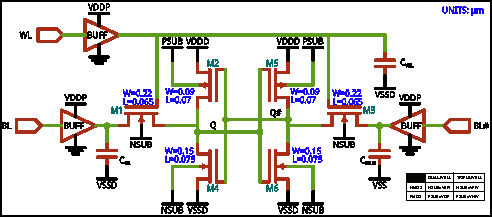
\includegraphics[width=1.0\textwidth]{./figures/sram_simulated.pdf}
\end{frame}

\begin{frame}{6T SRAM CELL CMOS\_065 functioning signals}
	\begin{columns}
		\begin{column}{0.5\textwidth}
			$(Q-\bar{Q})_{INIT}=L$
			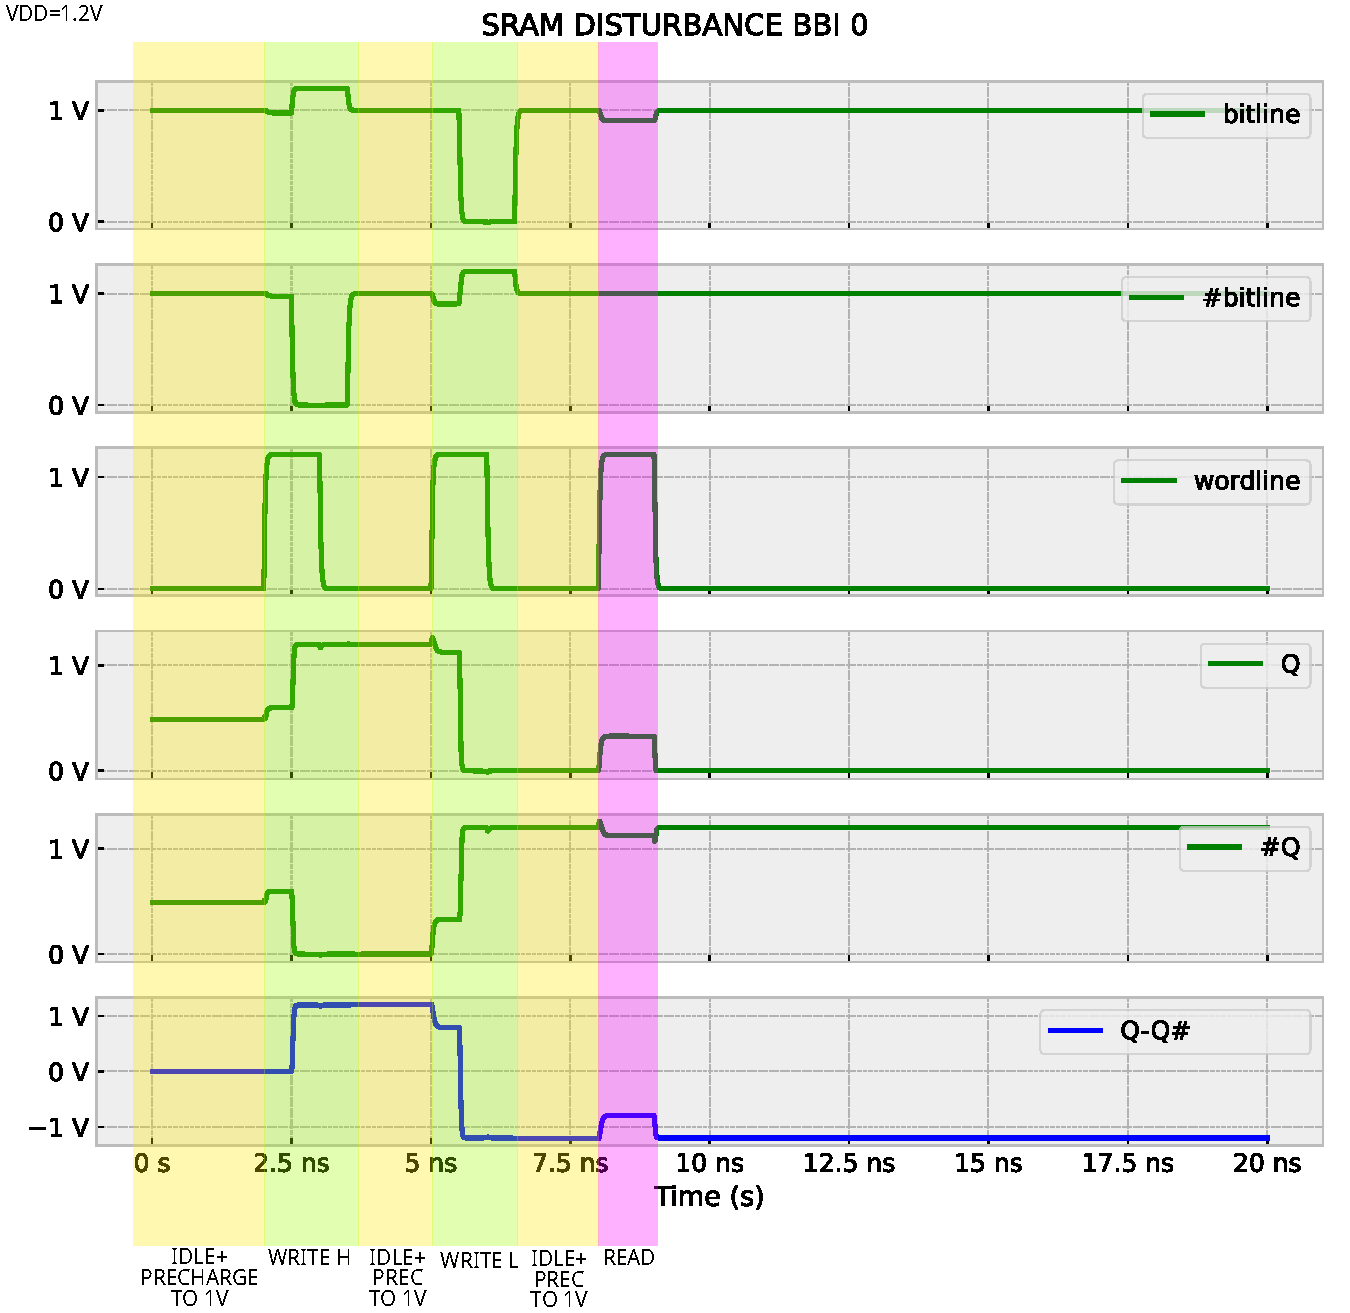
\includegraphics[width=\textwidth]{./figures/SRAMBBI0_zLOW.pdf}
		\end{column}
		\begin{column}{0.5\textwidth}
			$(Q-\bar{Q})_{INIT}=H$
			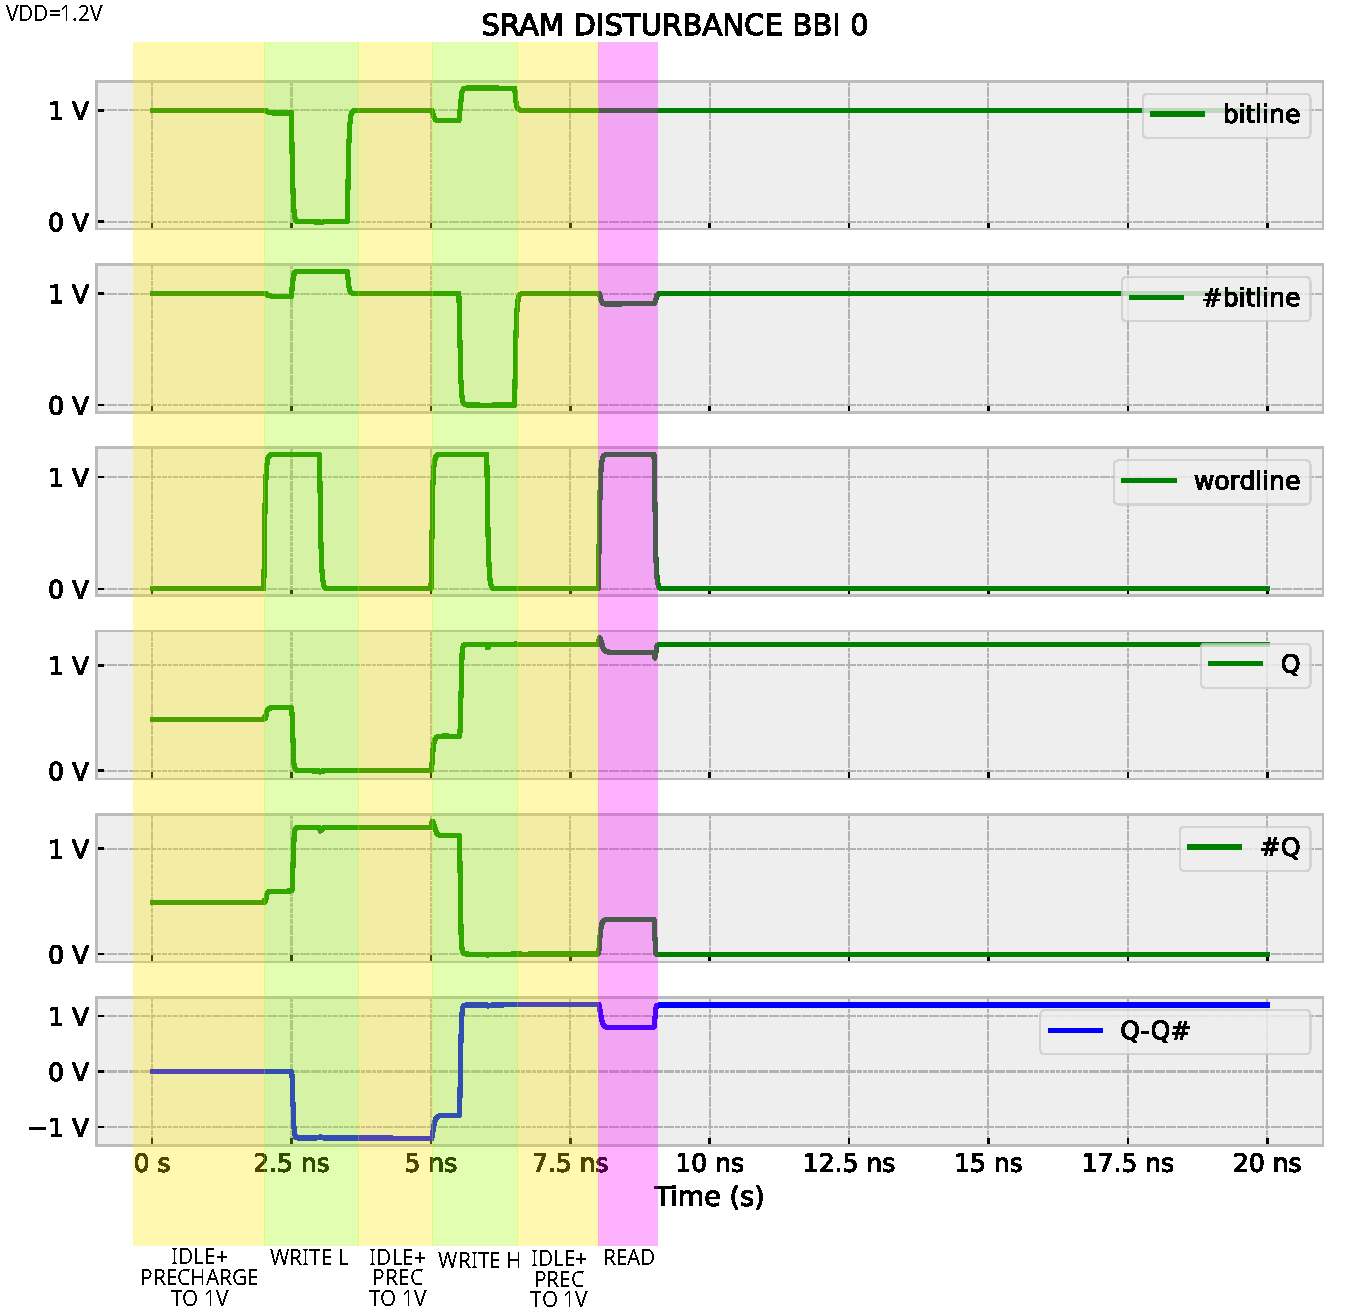
\includegraphics[width=\textwidth]{./figures/SRAMBBI0_zHIGH.pdf}
		\end{column}
	\end{columns}
\end{frame}

	% !TeX root = ./0_slides.tex

\begin{frame}{DUAL-WELL SUBSTRATE: OUT=H}
	\vspace{5mm}
	$(Q-\bar{Q})_{INIT}=H$
	\vspace{5mm}
	\begin{columns}
		\begin{column}{0.5\textwidth}
			\centering
%			\vspace{5mm}
			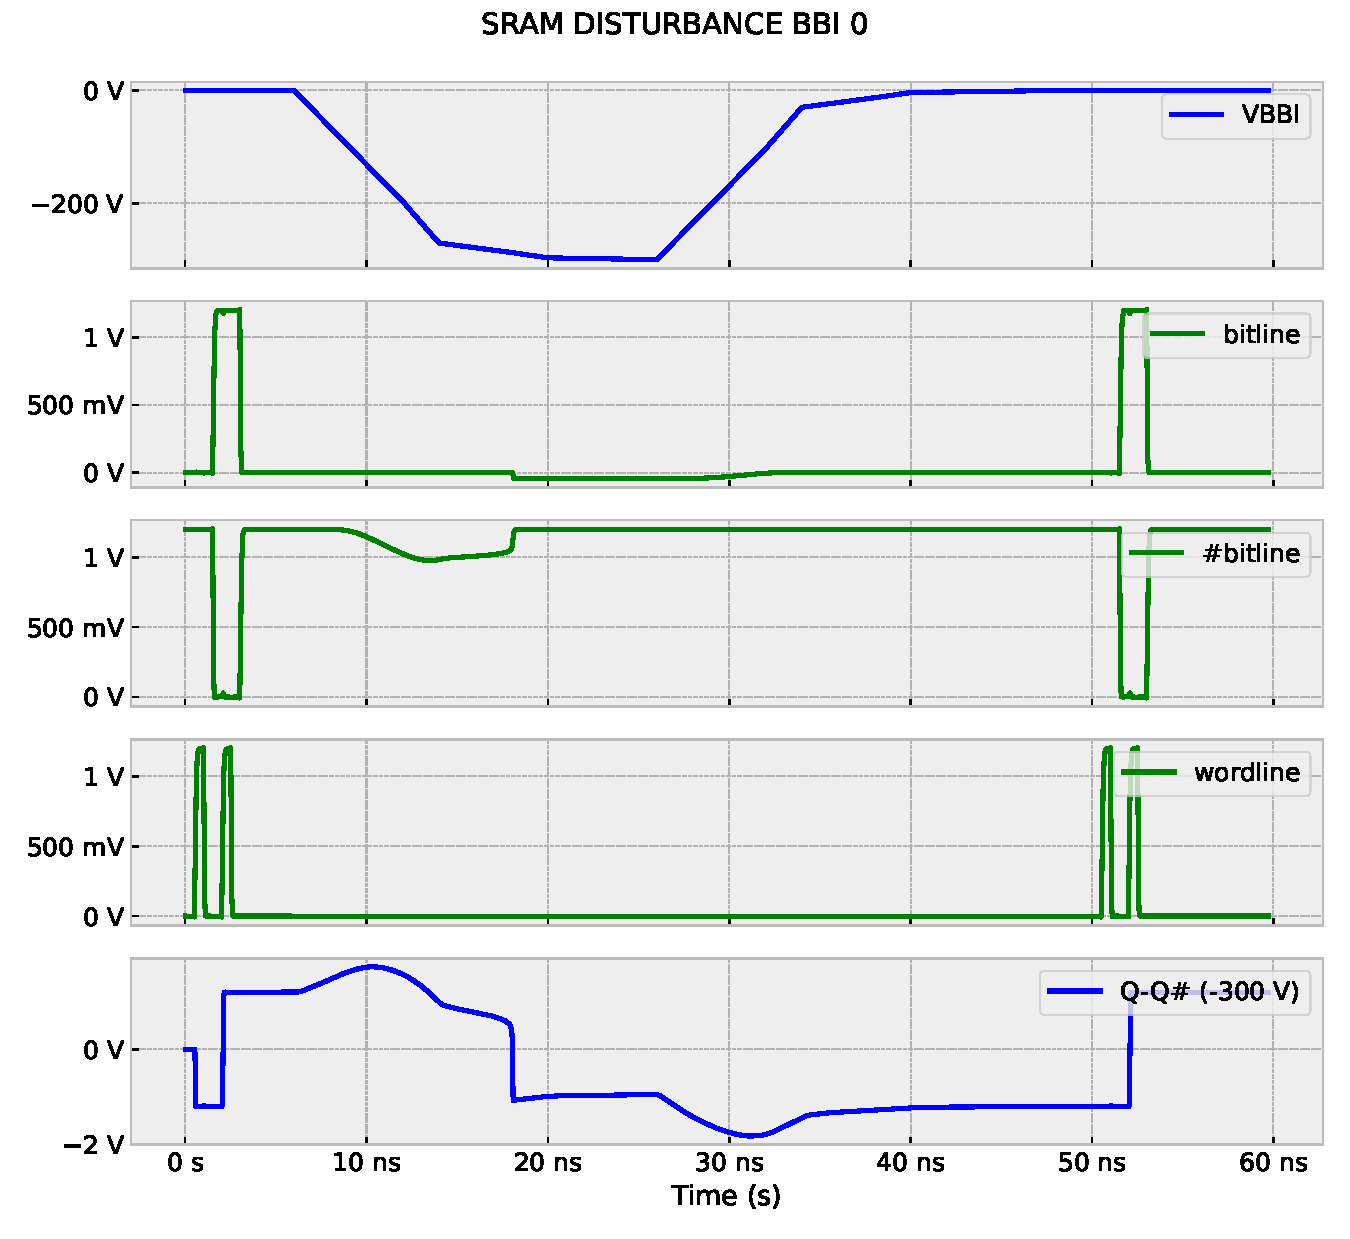
\includegraphics[width=\textwidth]{./figures/SRAMBBI0-300DW.pdf}
		\end{column}
		\begin{column}{0.5\textwidth}
			\centering
%			\vspace{5mm}
			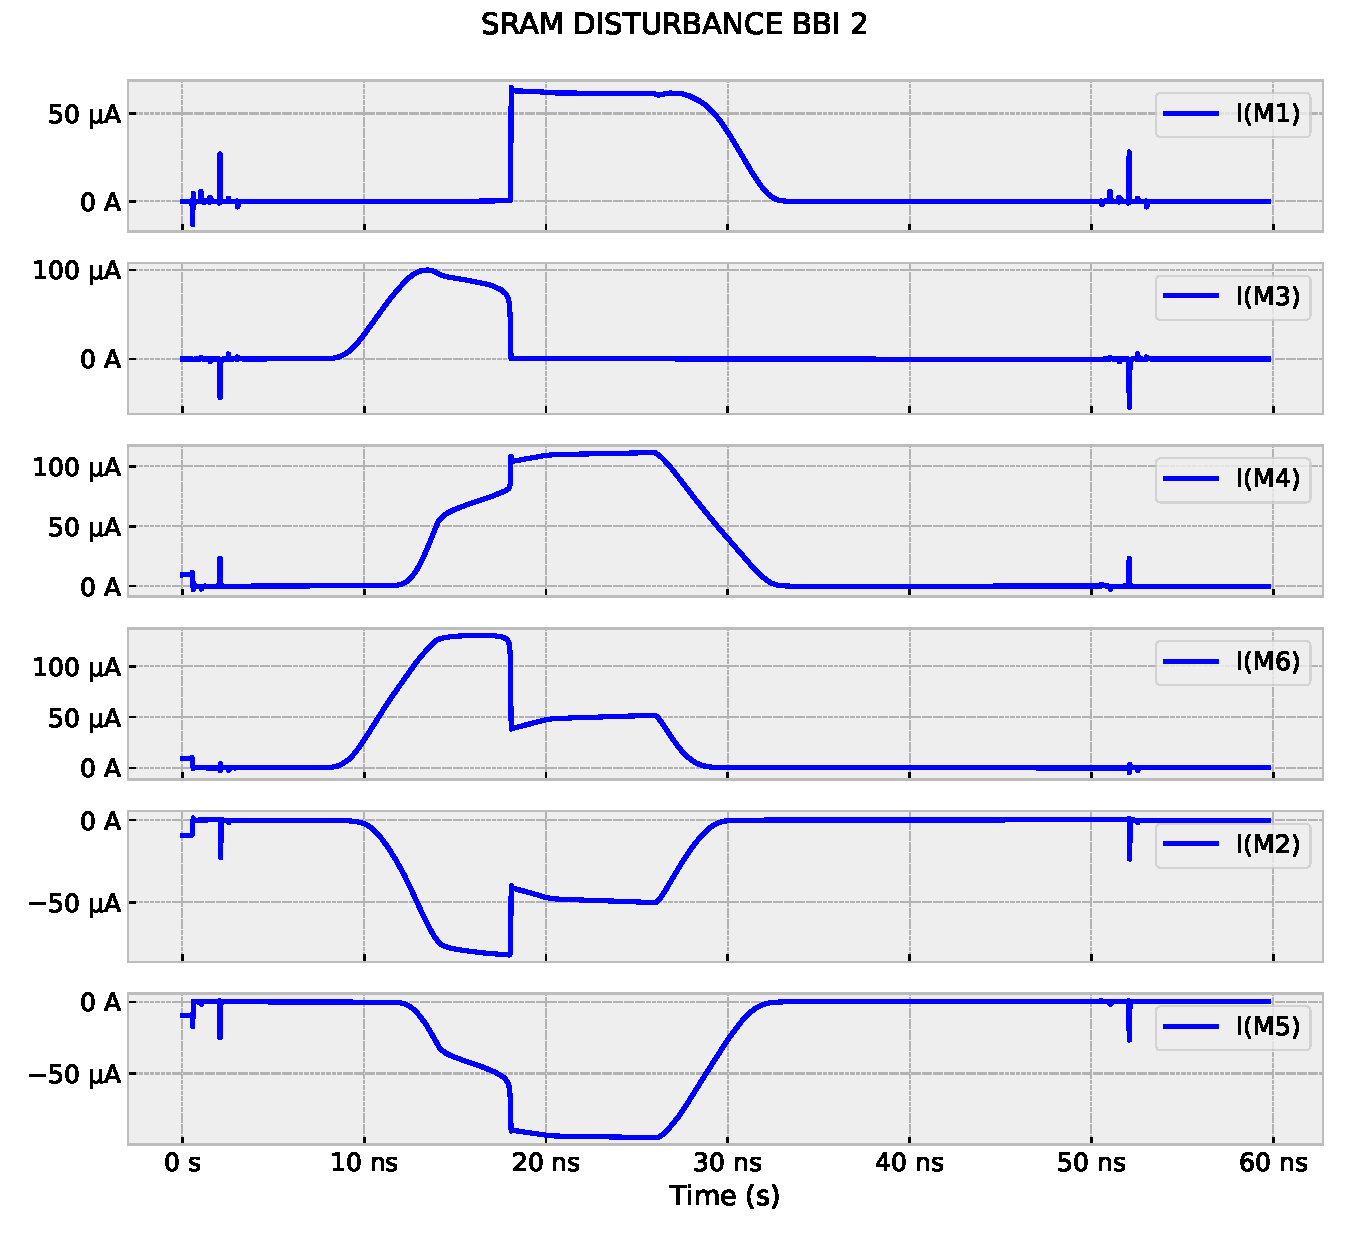
\includegraphics[width=\textwidth]{./figures/SRAMBBI2-300DW.pdf}
		\end{column}
	\end{columns}
\end{frame}

	% !TeX root = ./0_slides.tex

\begin{frame}{TRIPLE-WELL SUBSTRATE: OUT=H}
	\vspace{5mm}
	$(Q-\bar{Q})_{INIT}=H$
	\vspace{5mm}
	\begin{columns}
		\begin{column}{0.5\textwidth}
			\centering
%			\vspace{5mm}
			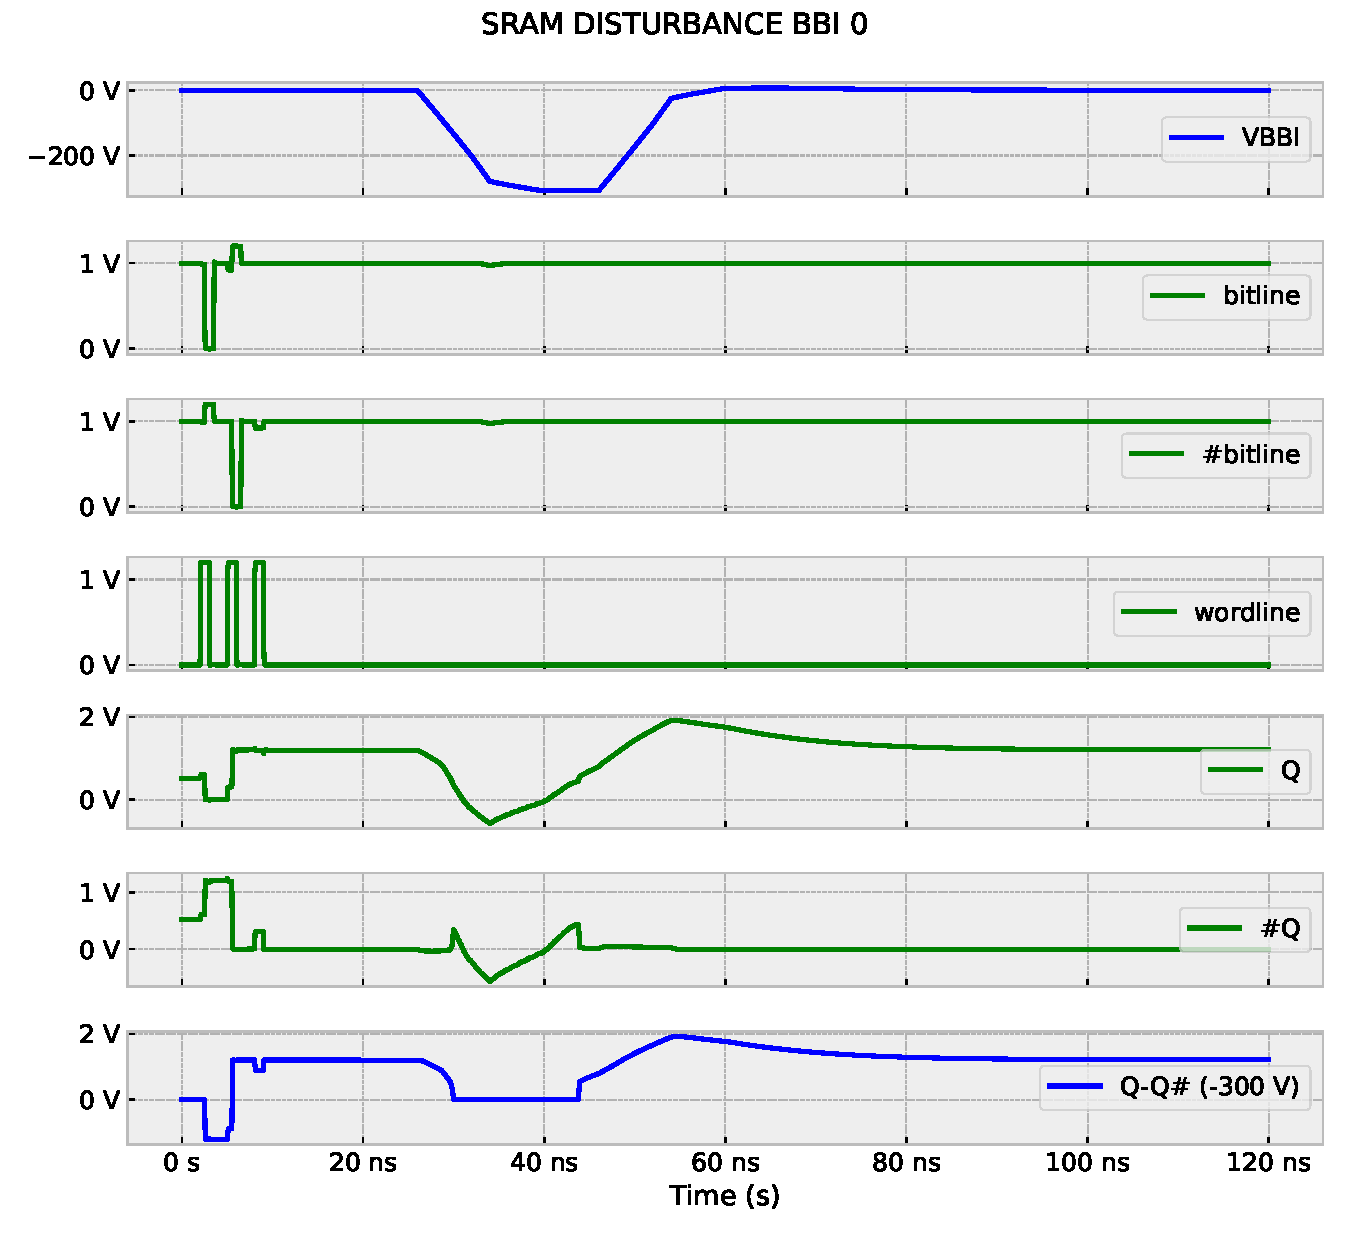
\includegraphics[width=\textwidth]{./figures/SRAMBBI0_zHIGH_TW-300.pdf}
		\end{column}
		\begin{column}{0.5\textwidth}
			\centering
%			\vspace{5mm}
			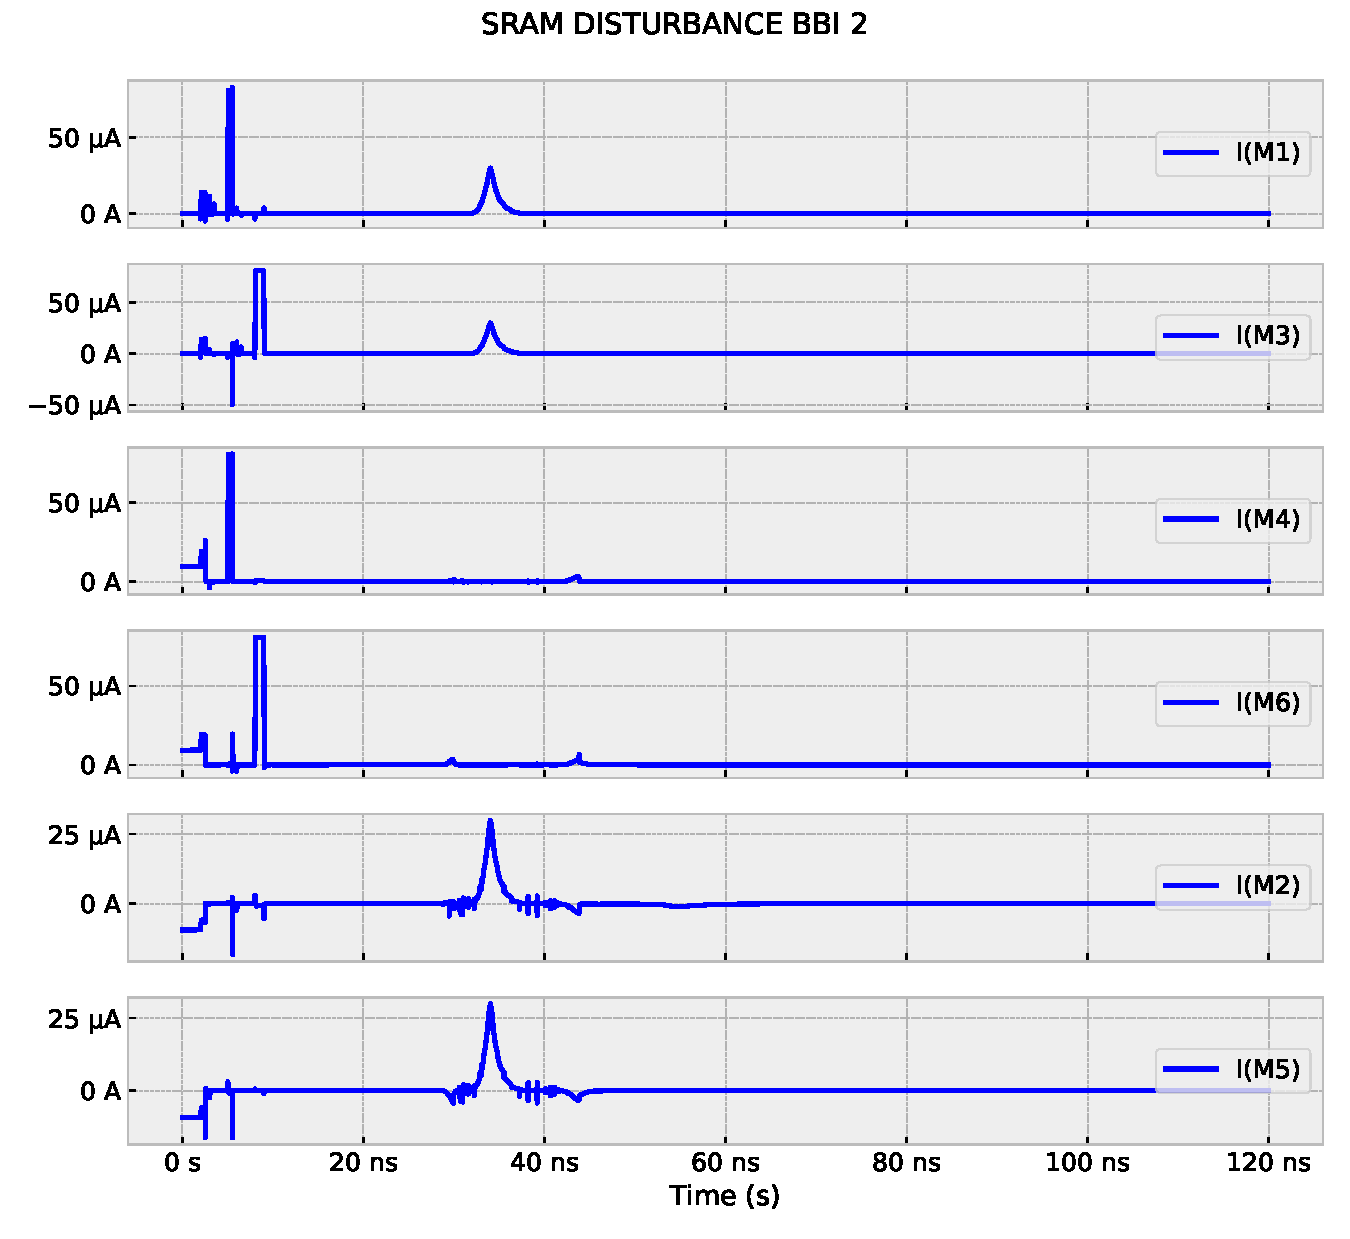
\includegraphics[width=\textwidth]{./figures/SRAMBBI2_zHIGH_TW-300.pdf}
		\end{column}
	\end{columns}
\end{frame}

	% !TeX root = ./0_slides.tex

\begin{frame}{DUAL-WELL SUBSTRATE: OUT=L}
	\vspace{5mm}
	$(Q-\bar{Q})_{INIT}=L$
	\vspace{5mm}
	\begin{columns}
		\begin{column}{0.5\textwidth}
			\centering
			%			\vspace{5mm}
			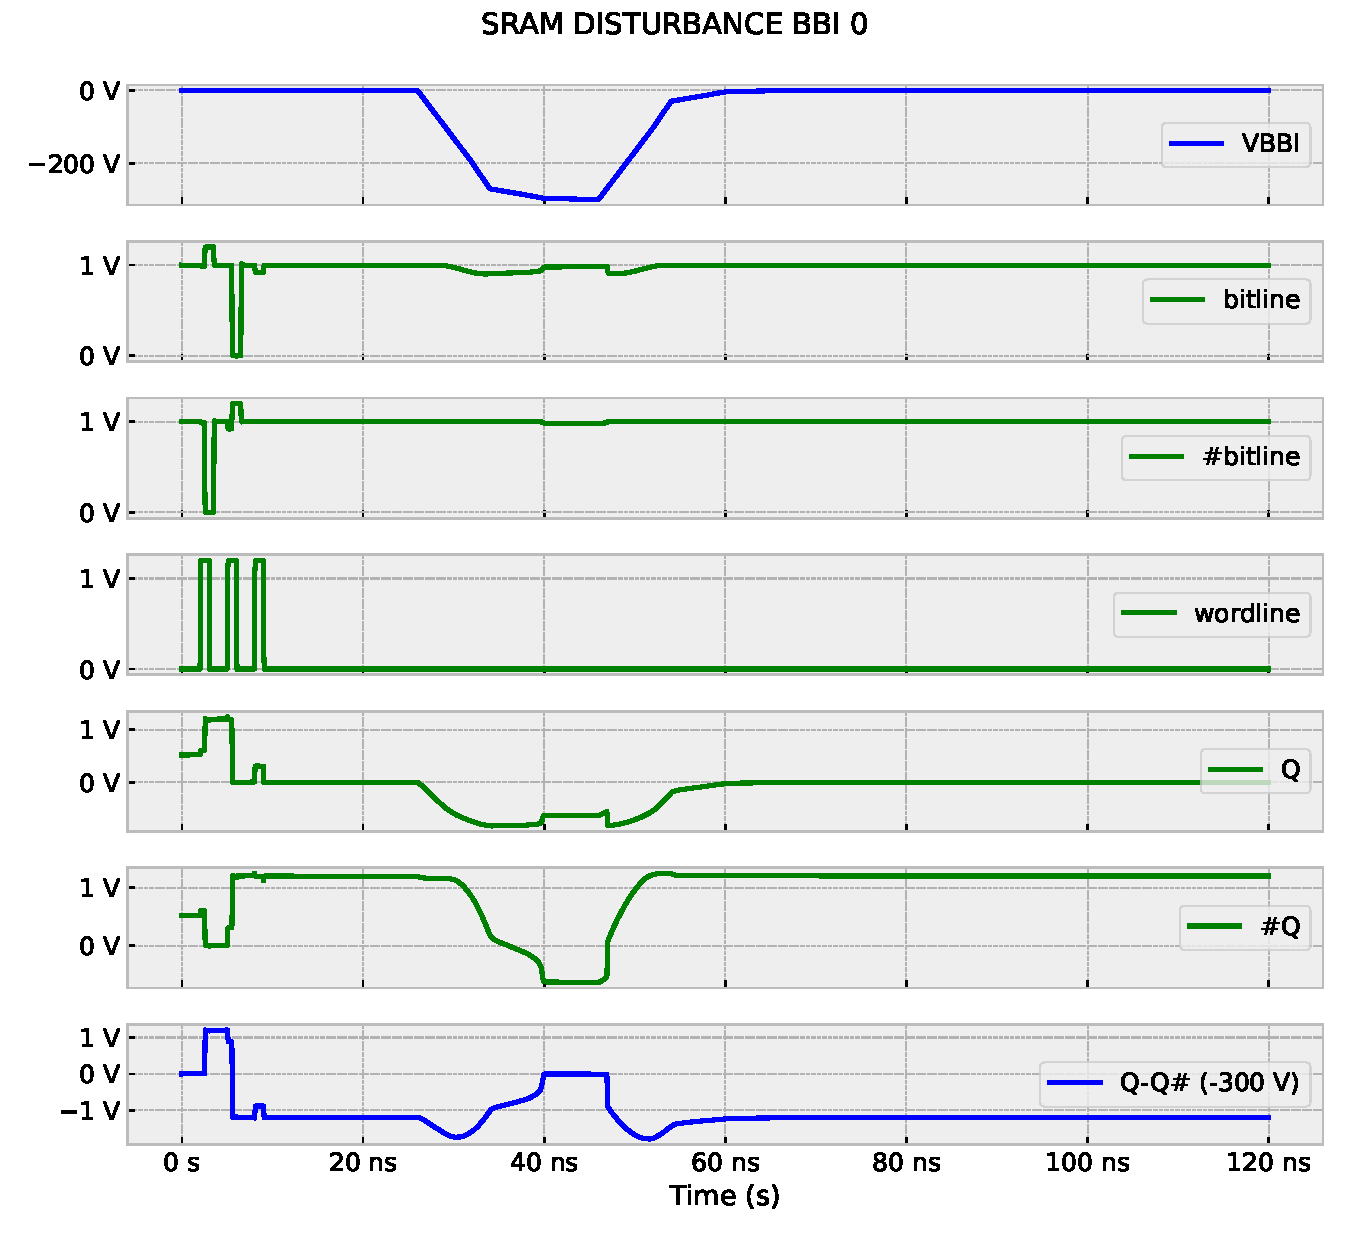
\includegraphics[width=\textwidth]{./figures/SRAMBBI0_zLOW_DW-300.pdf}
		\end{column}
		\begin{column}{0.5\textwidth}
			\centering
			%			\vspace{5mm}
			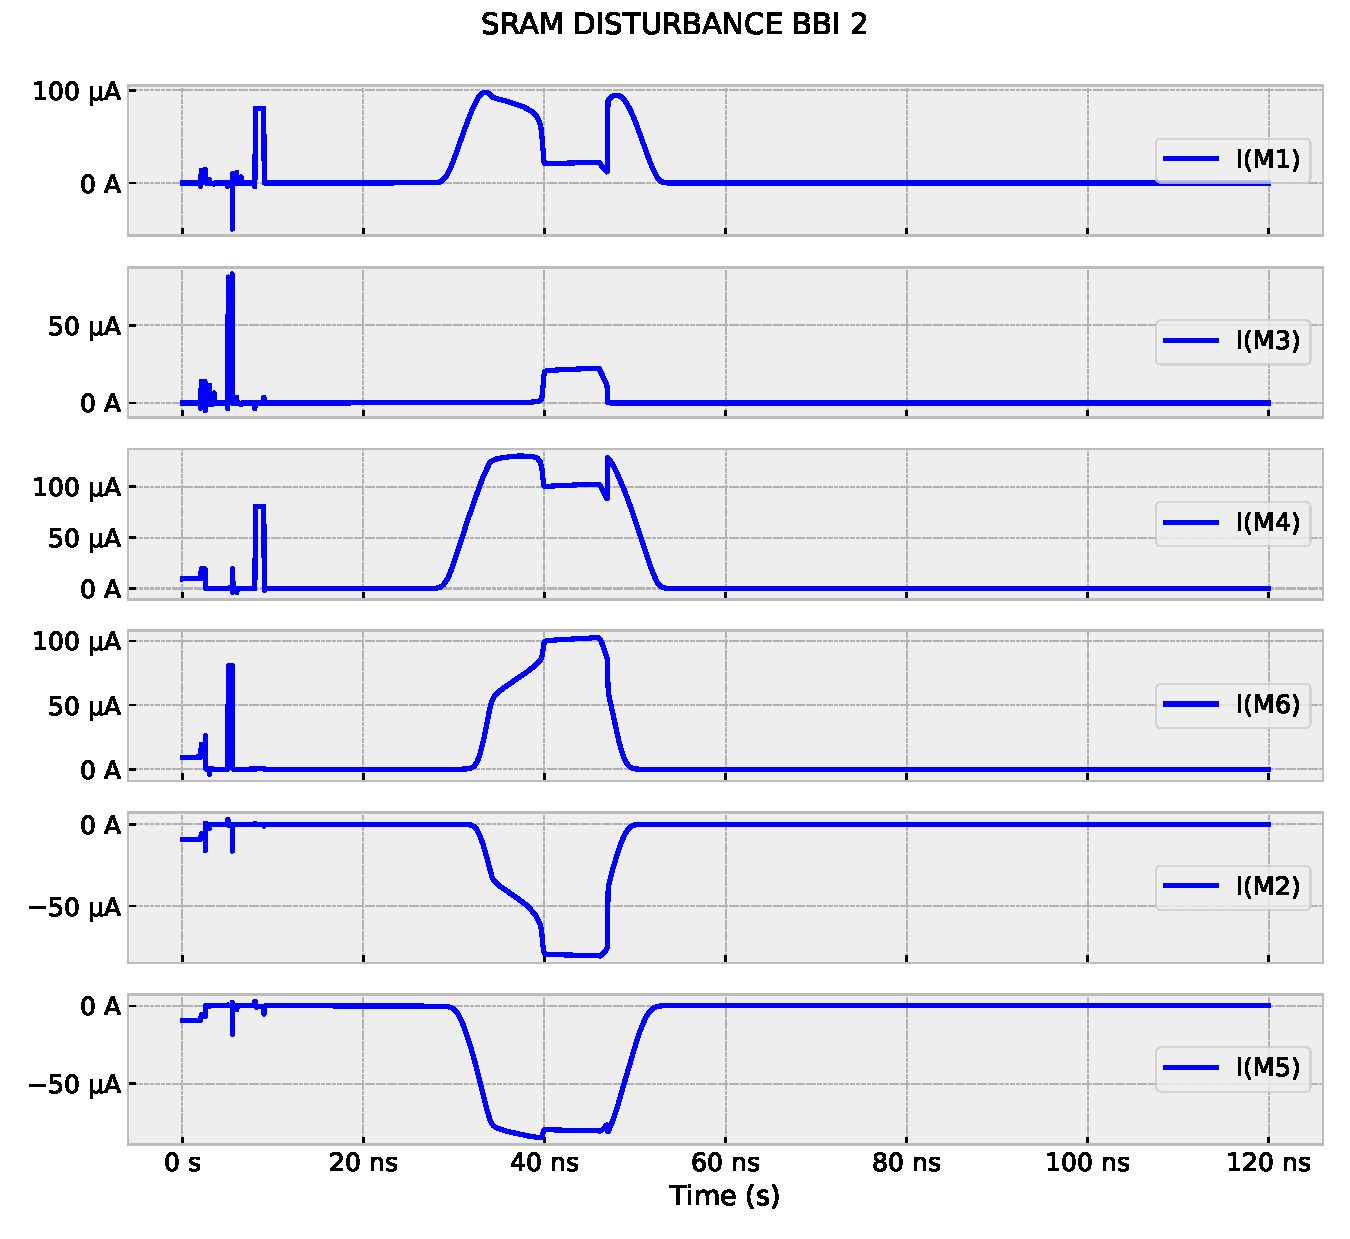
\includegraphics[width=\textwidth]{./figures/SRAMBBI2_zLOW_DW-300.pdf}
		\end{column}
	\end{columns}
\end{frame}

	% !TeX root = ./0_slides.tex

\begin{frame}{TRIPLE-WELL SUBSTRATE: OUT=L}
	\vspace{5mm}
	$(Q-\bar{Q})_{INIT}=L$
	\vspace{5mm}
	\begin{columns}
		\begin{column}{0.5\textwidth}
			\centering
			%			\vspace{5mm}
			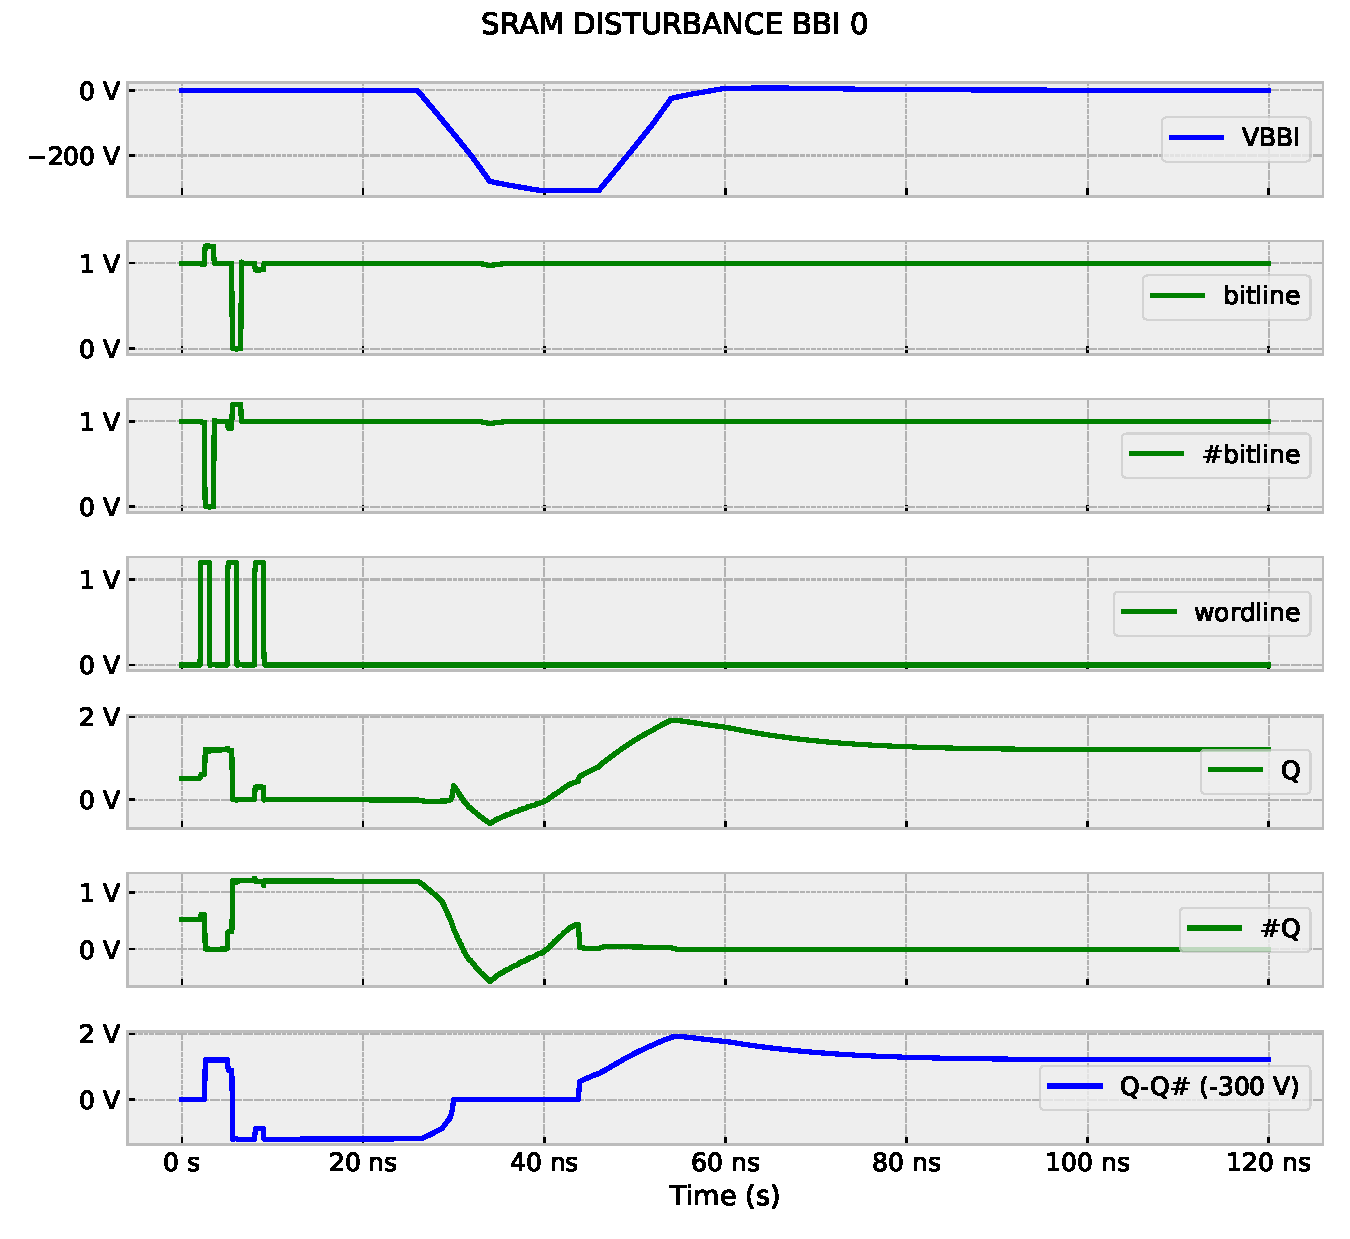
\includegraphics[width=\textwidth]{./figures/SRAMBBI0_zLOW_TW-300.pdf}
		\end{column}
		\begin{column}{0.5\textwidth}
			\centering
			%			\vspace{5mm}
			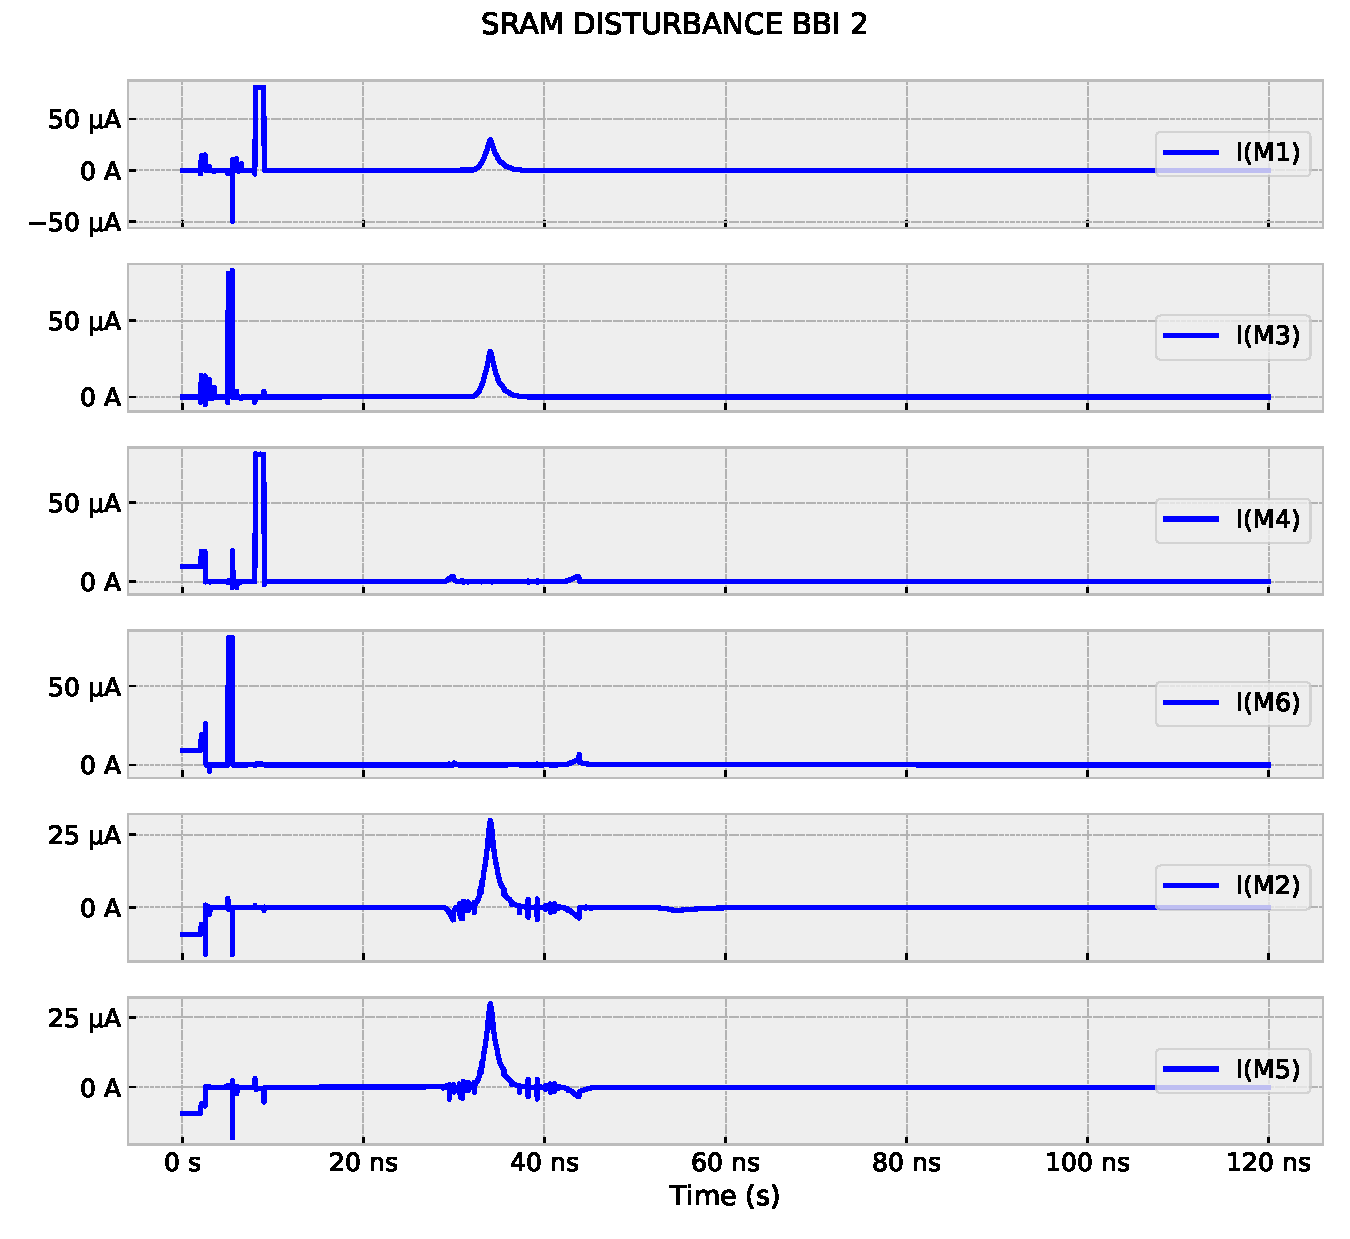
\includegraphics[width=\textwidth]{./figures/SRAMBBI2_zLOW_TW-300.pdf}
		\end{column}
	\end{columns}
\end{frame}

	
	% !TeX root = ./0_slides.tex

\section{IC THERMAL ANALYSIS}
%\begin{frame}{STM32 boot: 50 measurements on IC2}
%%	\centering
%%	\vspace{5mm}
%%	\includegraphics[width=0.9\textwidth]{./figures/beta0_ic2_50.pdf}
%%	\par
%%	20 reboots seems to be enough
%	\begin{columns}
%		\begin{column}{0.7\textwidth}
%			\includegraphics[width=.9\textwidth]{./figures/flistCircuit2_50_sl30.pdf}
%		\end{column}
%		\begin{column}{0.3\textwidth}
%			20 reboots \textrightarrow\ enough
%		\end{column}
%	\end{columns}
%\end{frame}

	% !TeX root = ./0_slides.tex

\begin{frame}{STM32 boot: IC1 \textrightarrow\ Opened}
	\vspace{5mm}
	\begin{columns}
		\begin{column}{0.5\textwidth}
			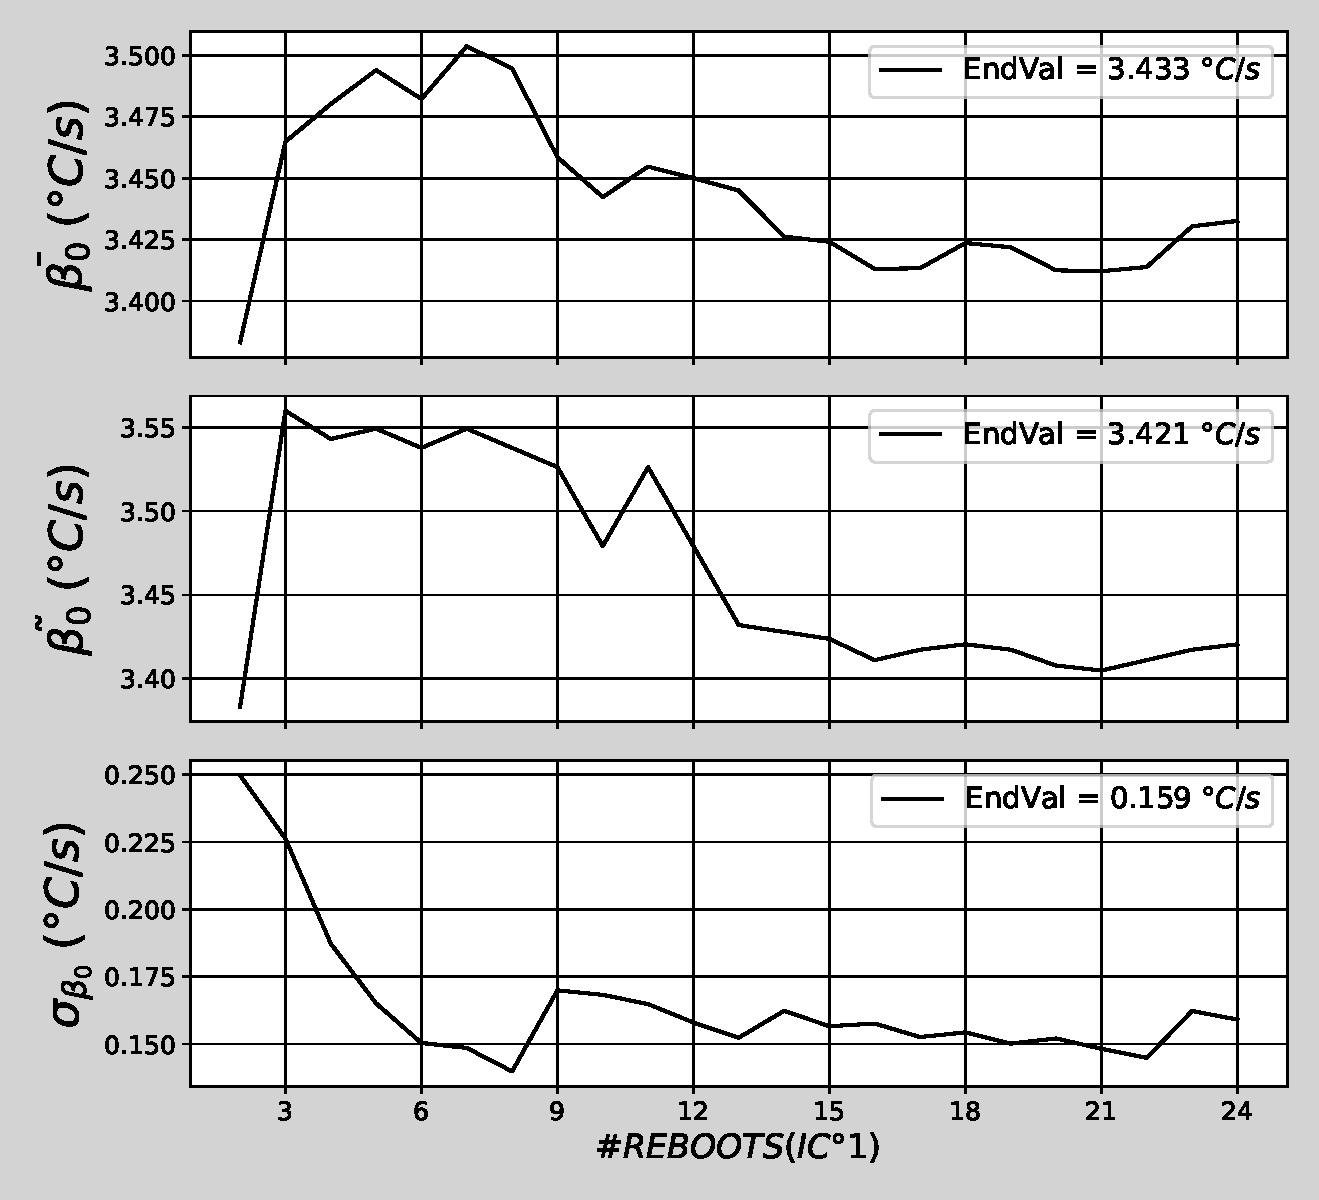
\includegraphics[width=1.0\textwidth]{./figures/flistCircuit1_25_sl30beta0.pdf}
		\end{column}
		\begin{column}{0.5\textwidth}
			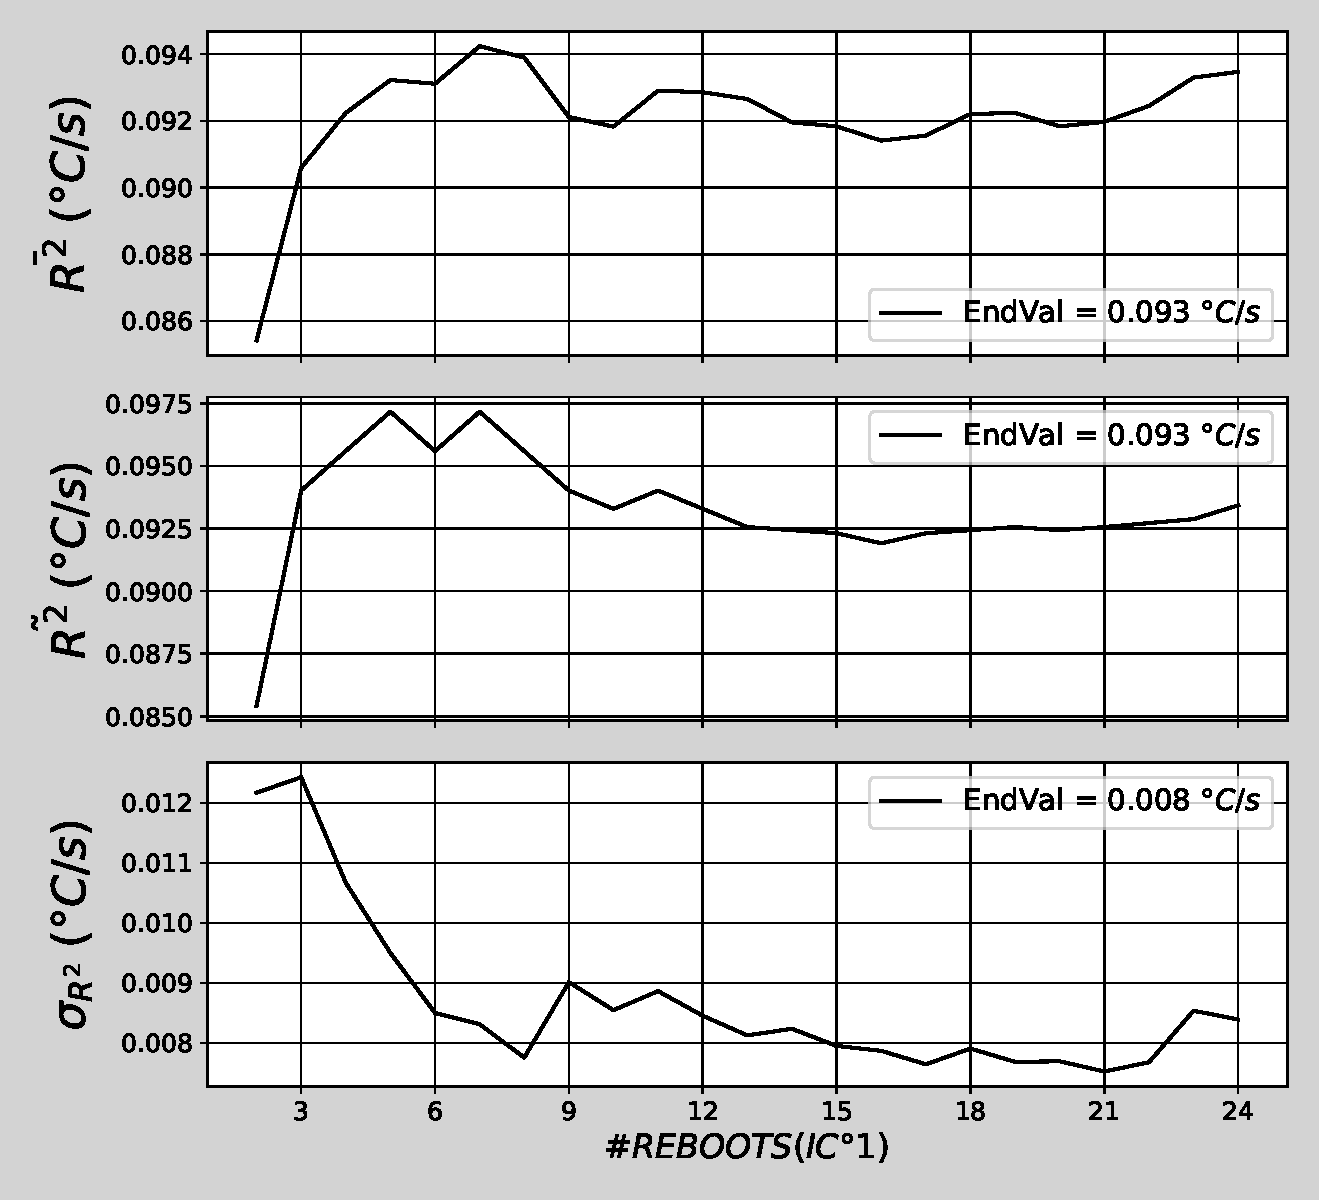
\includegraphics[width=1.0\textwidth]{./figures/flistCircuit1_25_sl30r2.pdf}
		\end{column}
	\end{columns}
\end{frame}

\begin{frame}{STM32 boot: IC2 \textrightarrow\ Normal}
	\vspace{5mm}
	\begin{columns}
		\begin{column}{0.5\textwidth}
			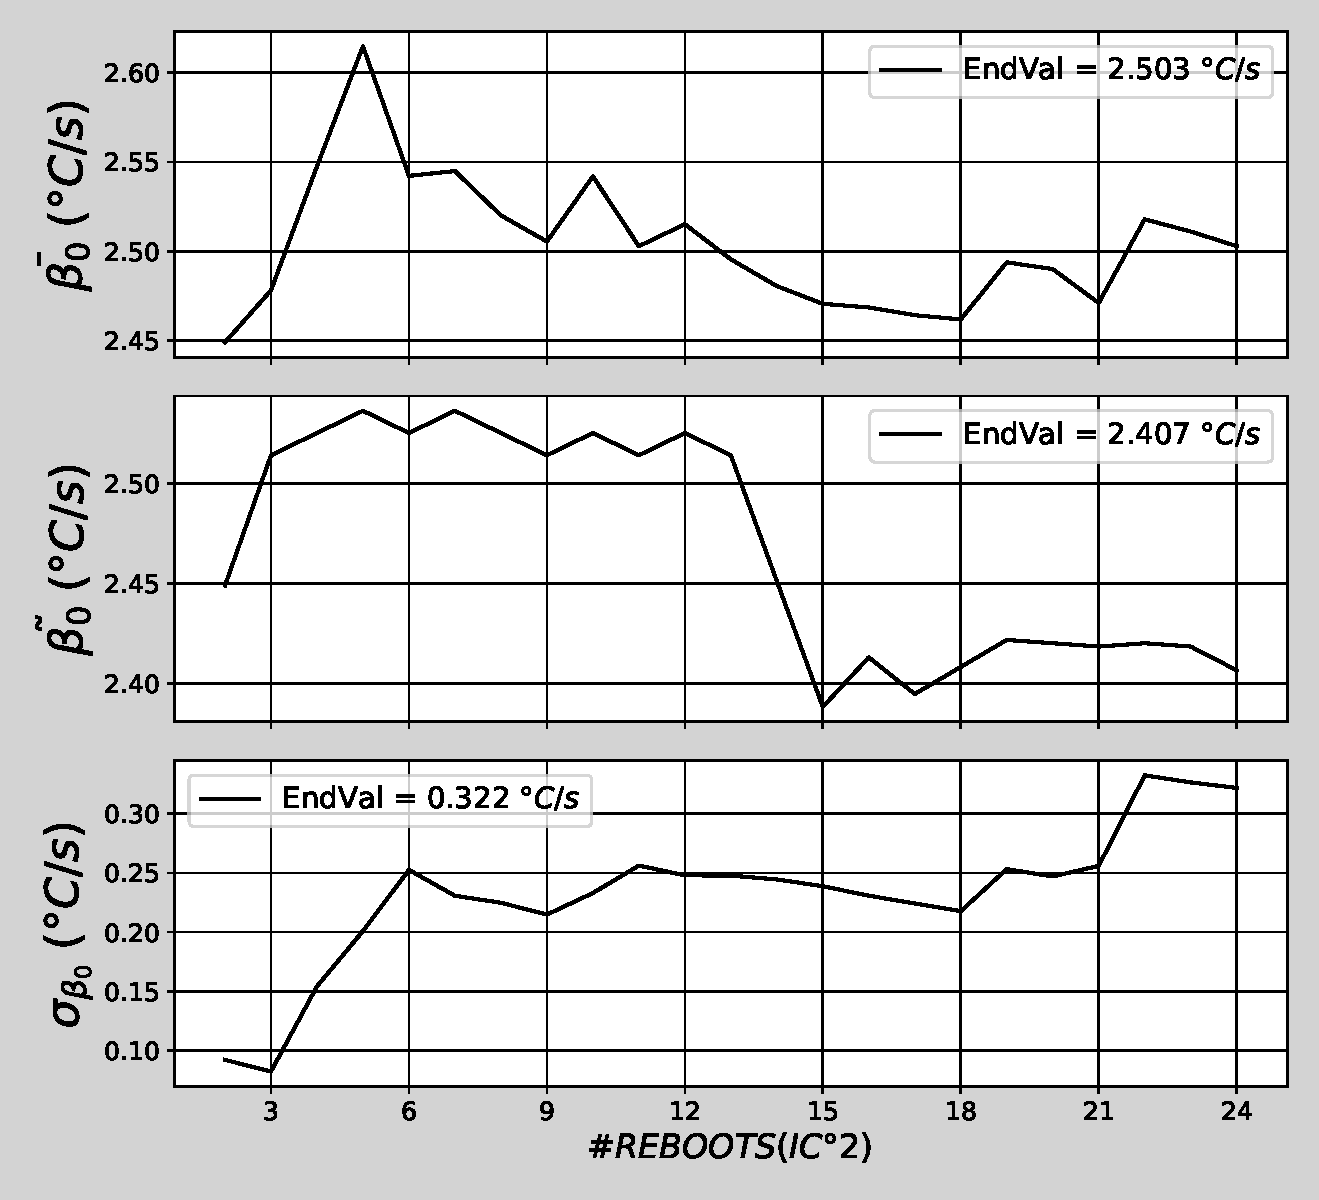
\includegraphics[width=1.0\textwidth]{./figures/flistCircuit2_25_sl30_2beta0.pdf}
		\end{column}
		\begin{column}{0.5\textwidth}
			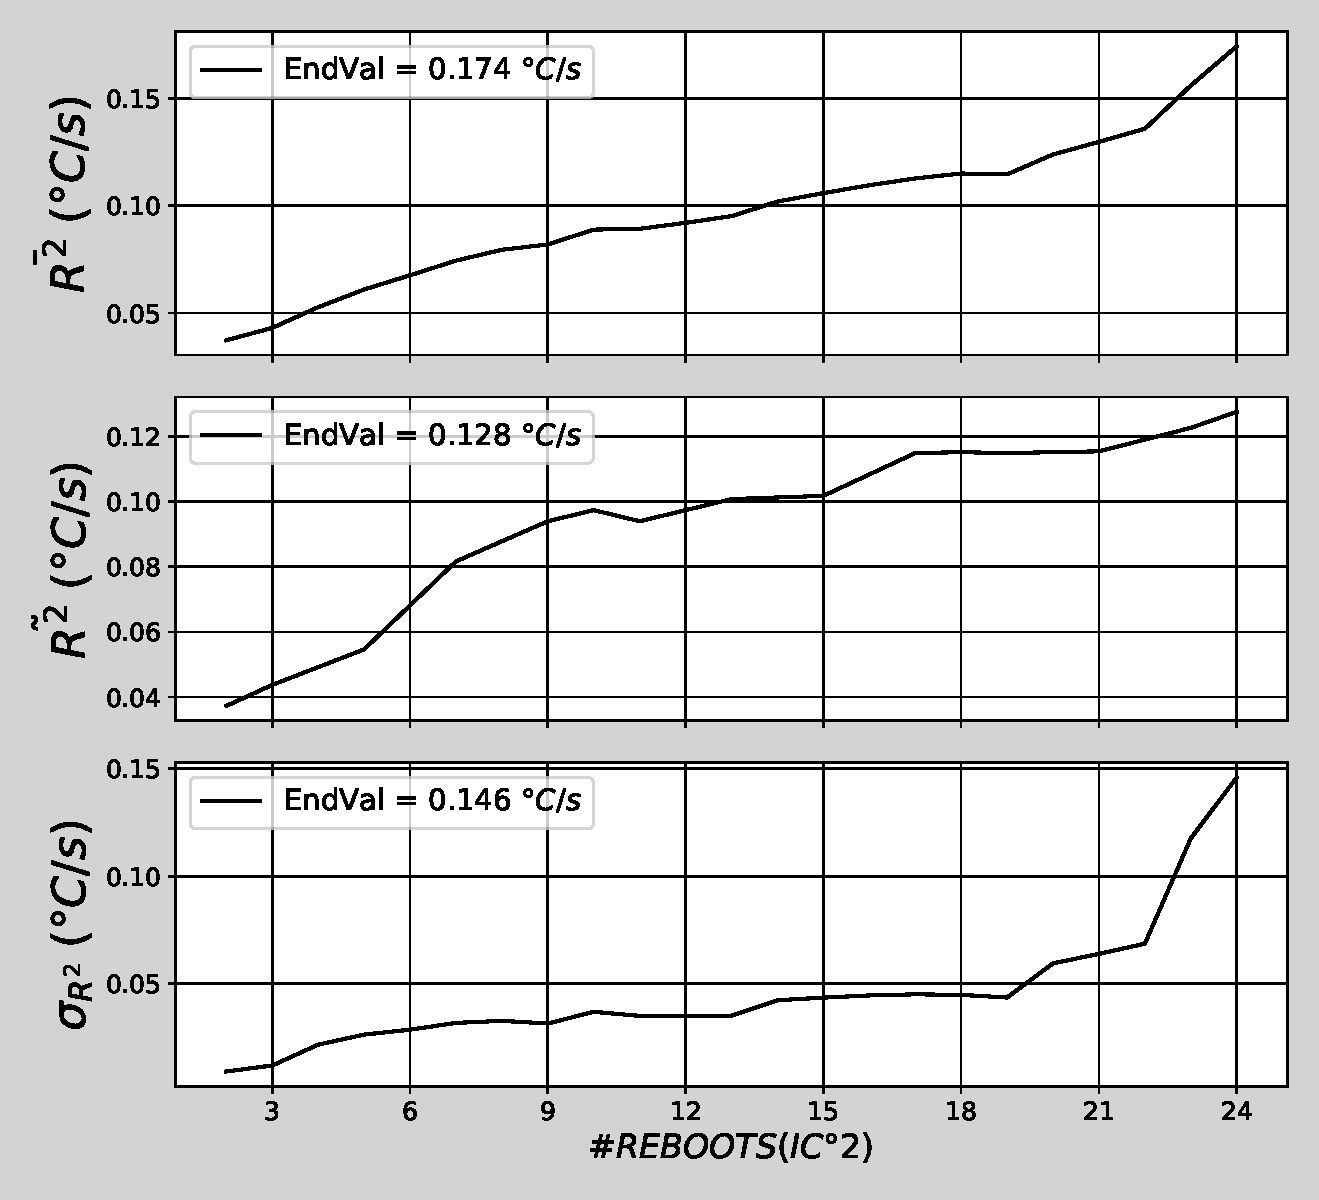
\includegraphics[width=1.0\textwidth]{./figures/flistCircuit2_25_sl30_2r2.pdf}
		\end{column}
	\end{columns}
\end{frame}

\begin{frame}{STM32 boot: IC3 \textrightarrow\ Closed}
	\vspace{5mm}
	\begin{columns}
		\begin{column}{0.5\textwidth}
			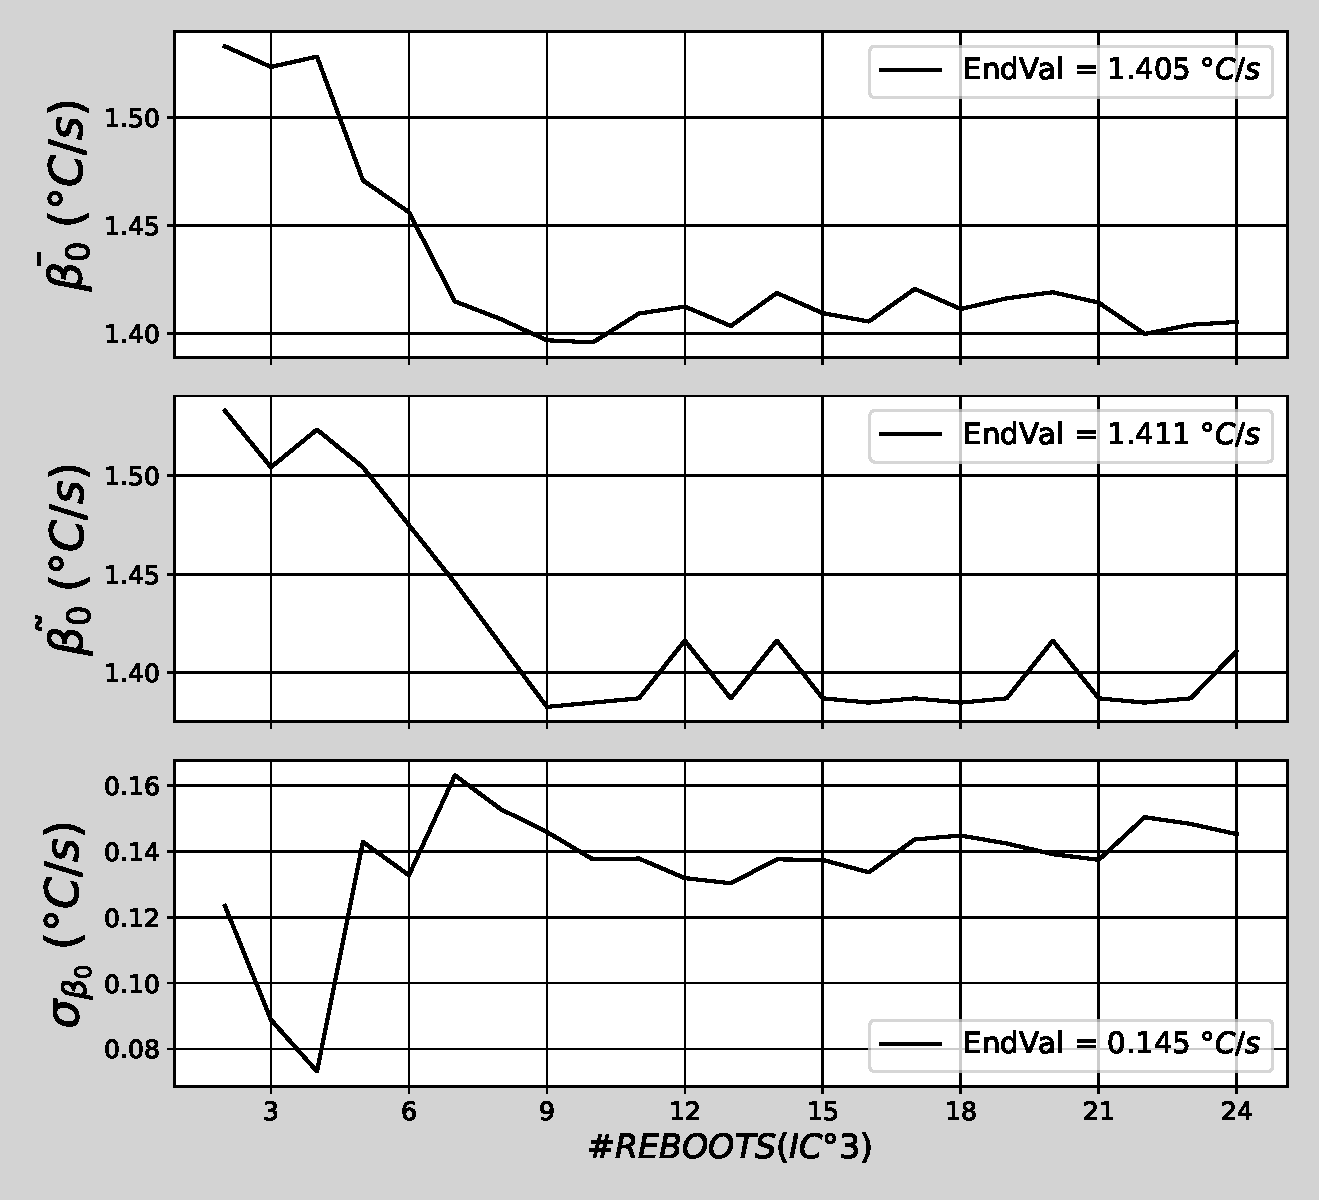
\includegraphics[width=1.0\textwidth]{./figures/flistCircuit3_25_sl30beta0.pdf}
		\end{column}
		\begin{column}{0.5\textwidth}
			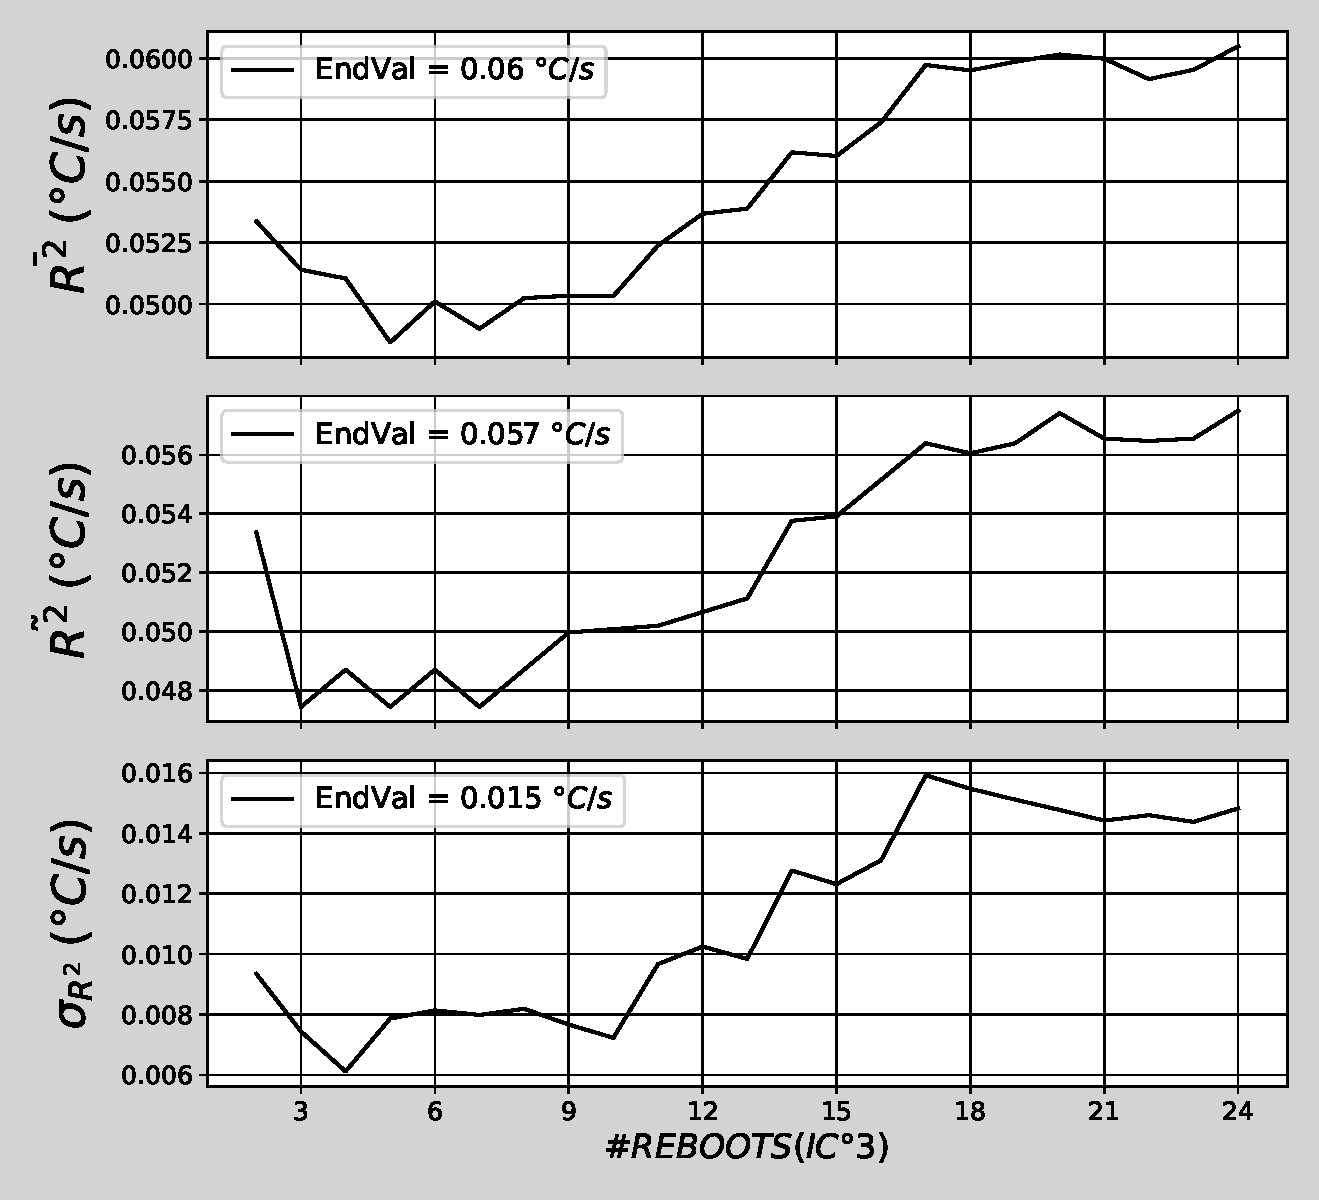
\includegraphics[width=1.0\textwidth]{./figures/flistCircuit3_25_sl30r2.pdf}
		\end{column}
	\end{columns}
\end{frame}

\begin{frame}{STM32 boot: IC4 \textrightarrow\ Opened}
	\vspace{5mm}
	\begin{columns}
		\begin{column}{0.5\textwidth}
			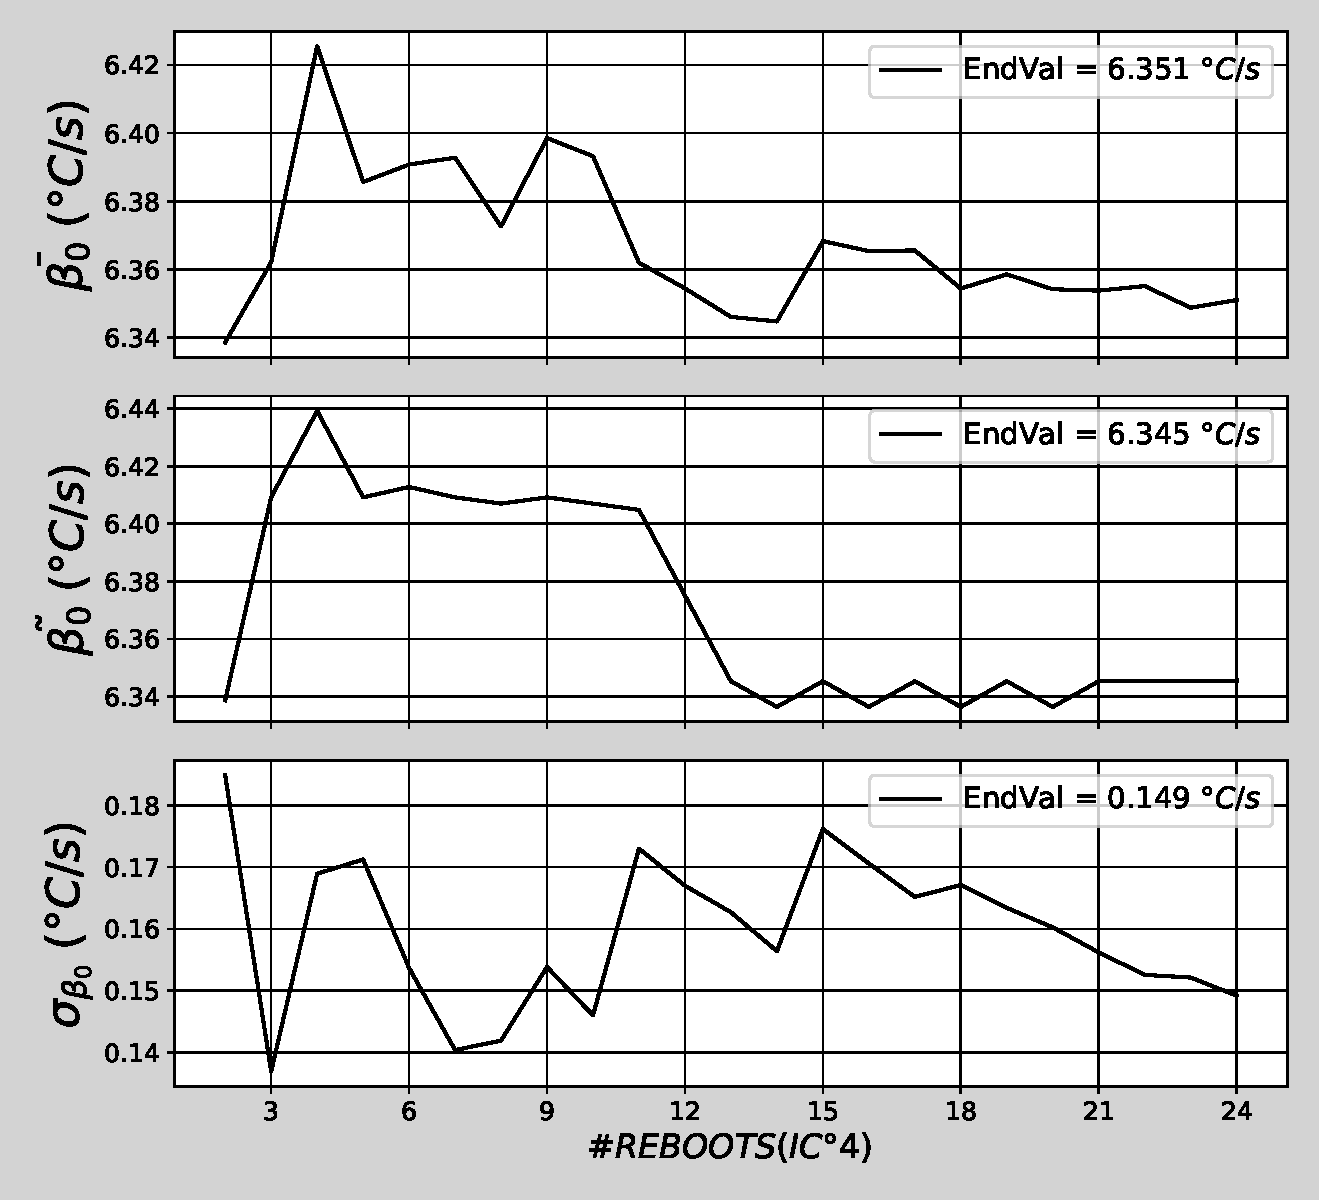
\includegraphics[width=1.0\textwidth]{./figures/flistCircuit4_25_sl30beta0.pdf}
		\end{column}
		\begin{column}{0.5\textwidth}
			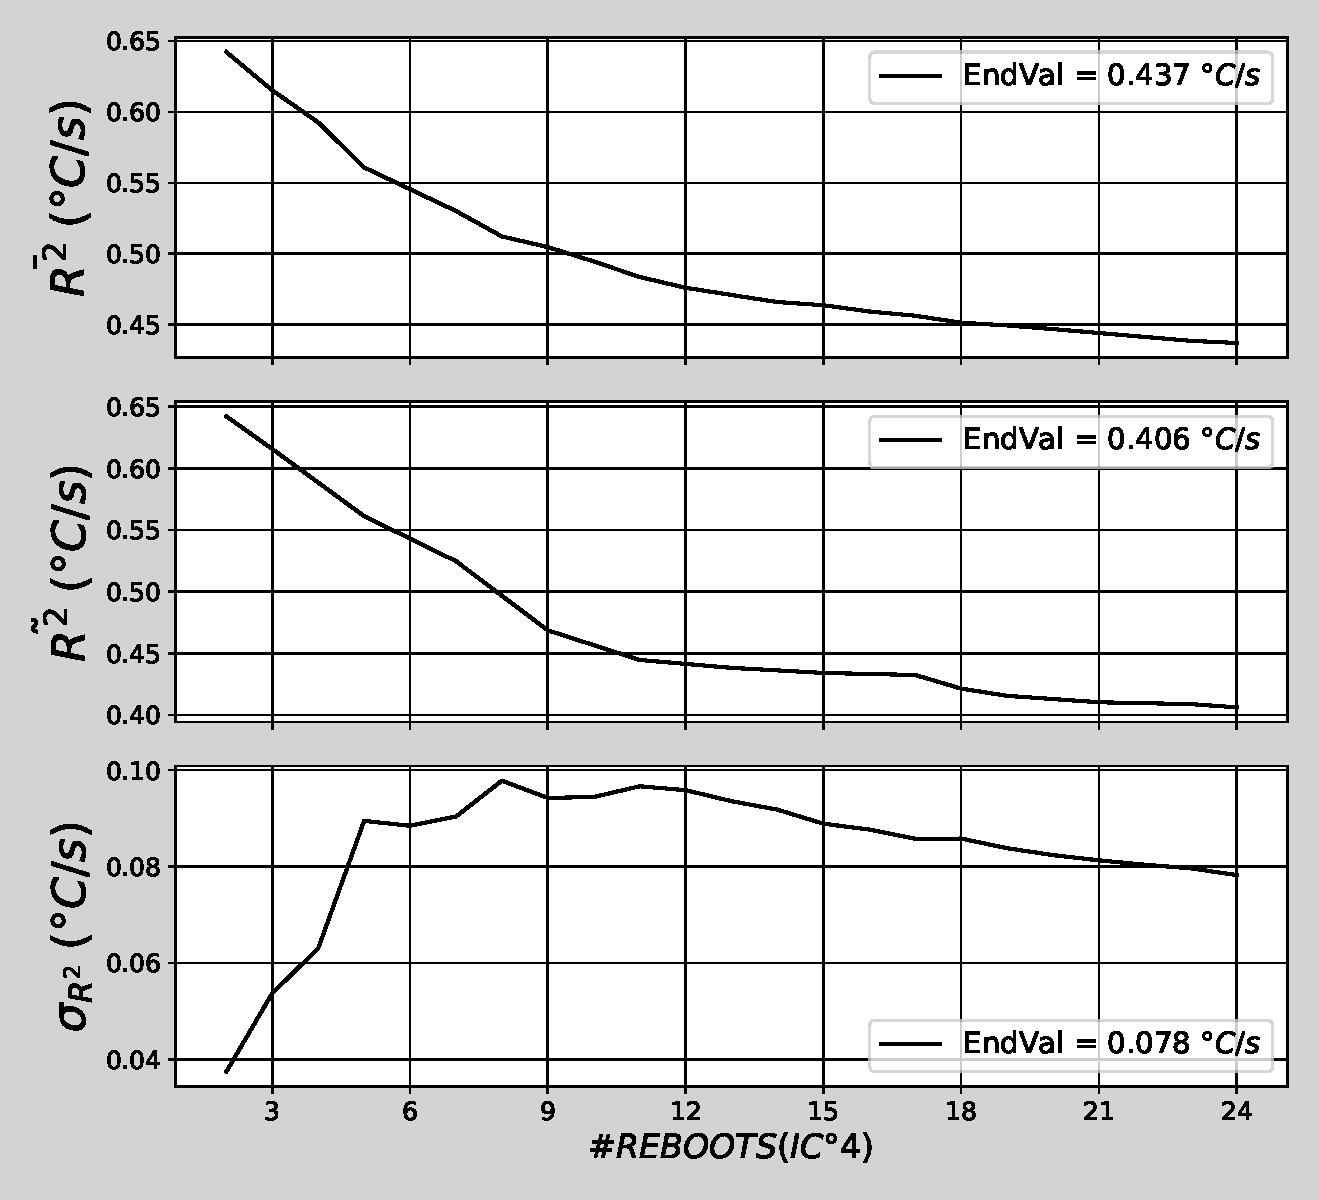
\includegraphics[width=1.0\textwidth]{./figures/flistCircuit4_25_sl30r2.pdf}
		\end{column}
	\end{columns}
\end{frame}

\begin{frame}{STM32 boot: IC6 \textrightarrow\ Closed}
	\vspace{5mm}
	\begin{columns}
		\begin{column}{0.5\textwidth}
			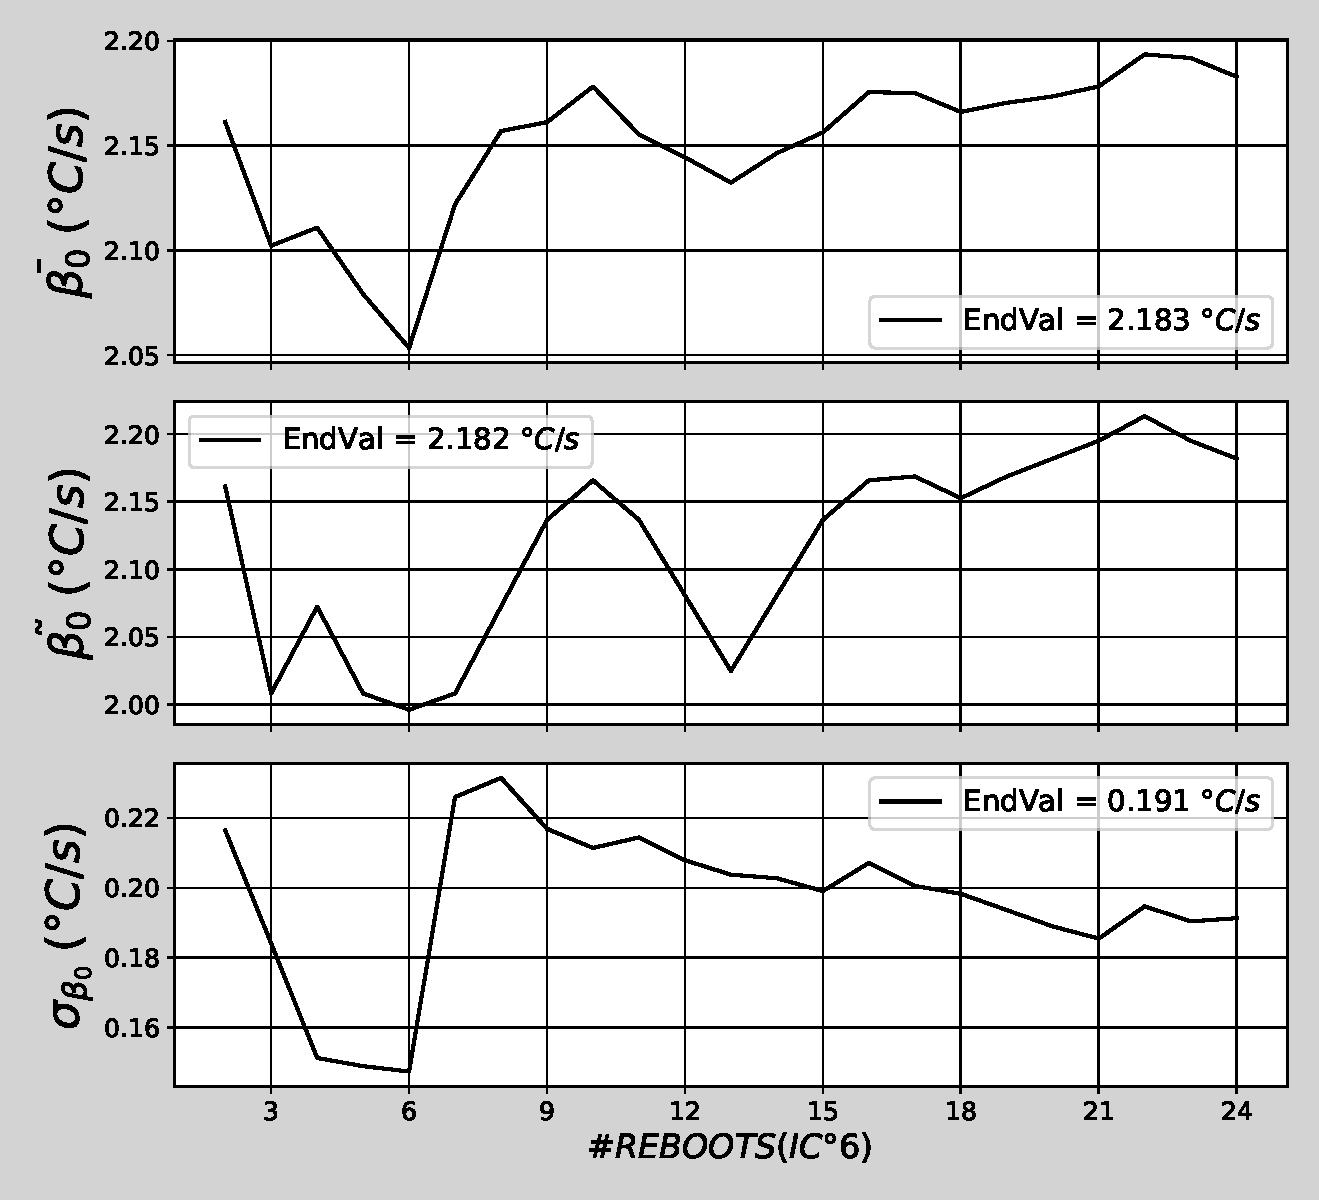
\includegraphics[width=1.0\textwidth]{./figures/flistCircuit6_25_sl30beta0.pdf}
		\end{column}
		\begin{column}{0.5\textwidth}
			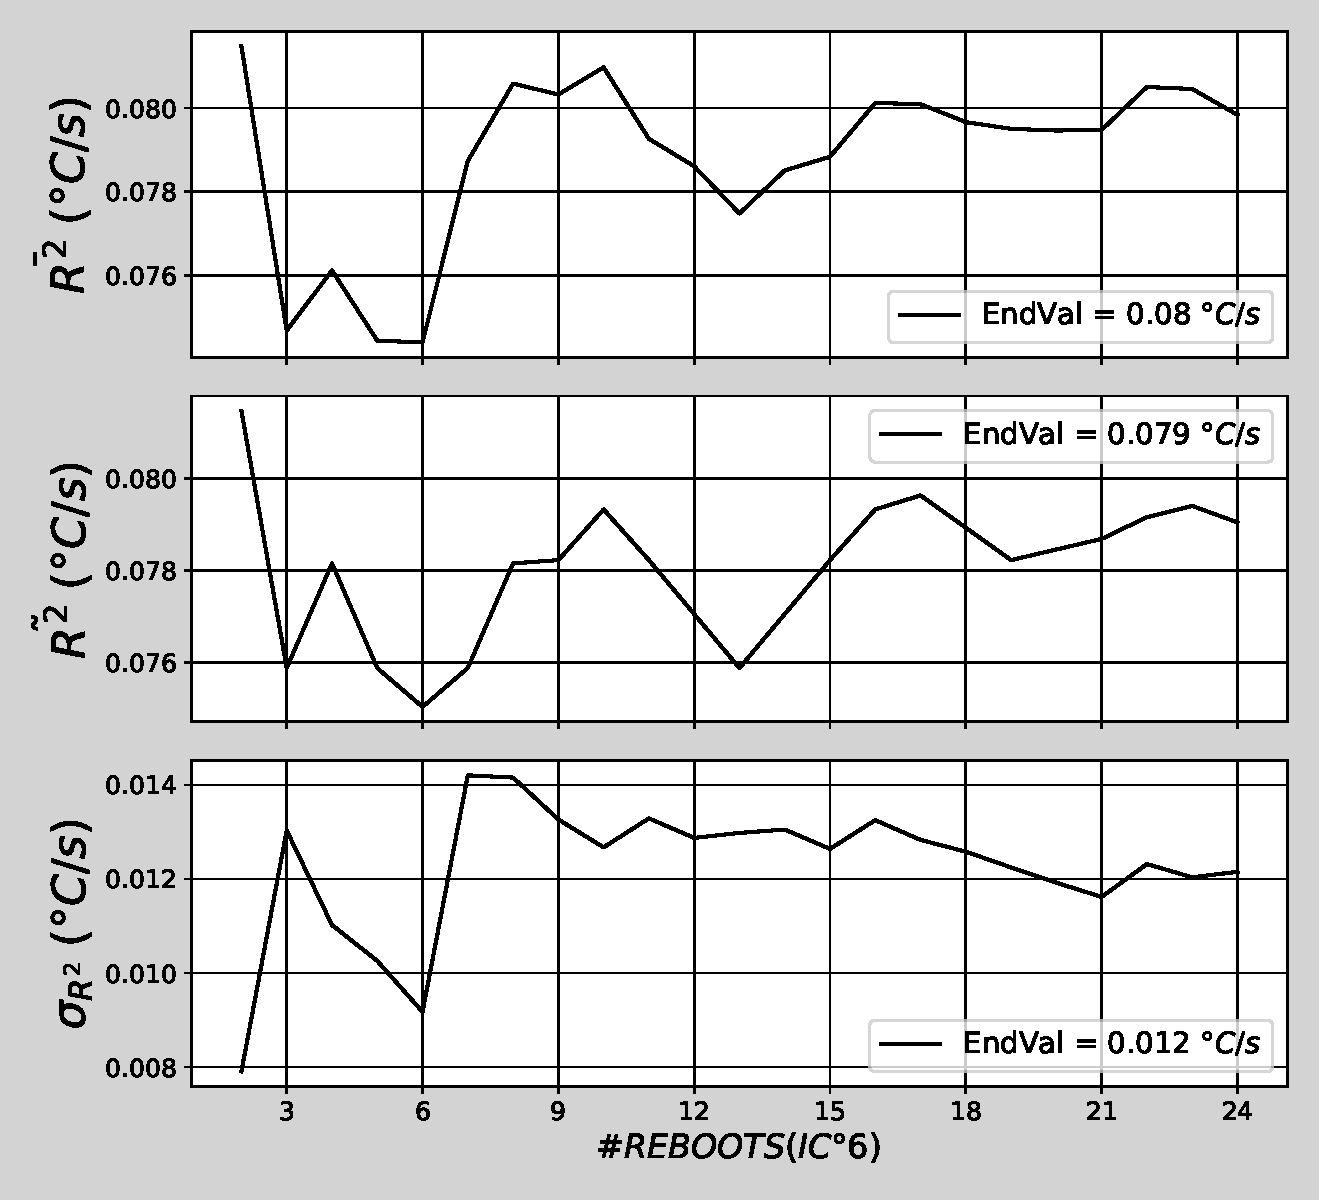
\includegraphics[width=1.0\textwidth]{./figures/flistCircuit6_25_sl30r2.pdf}
		\end{column}
	\end{columns}
\end{frame}

\begin{frame}{STM32 boot: IC7 \textrightarrow\ Opened}
	\vspace{5mm}
	\begin{columns}
		\begin{column}{0.5\textwidth}
			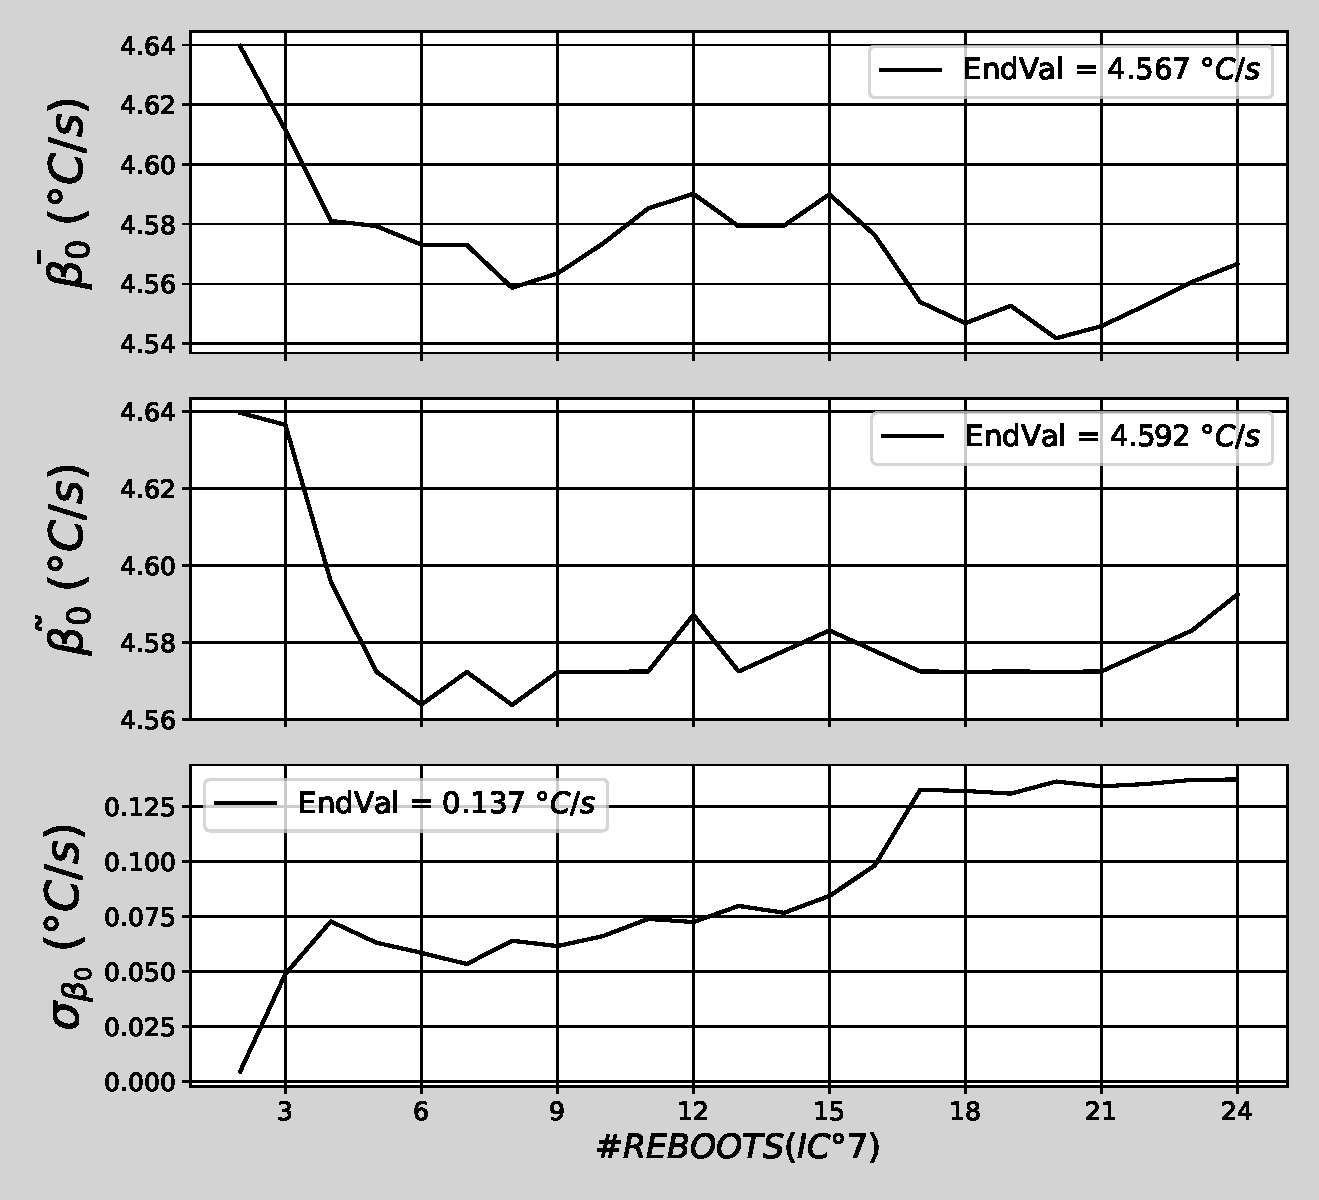
\includegraphics[width=1.0\textwidth]{./figures/flistCircuit7_25_sl30beta0.pdf}
		\end{column}
		\begin{column}{0.5\textwidth}
			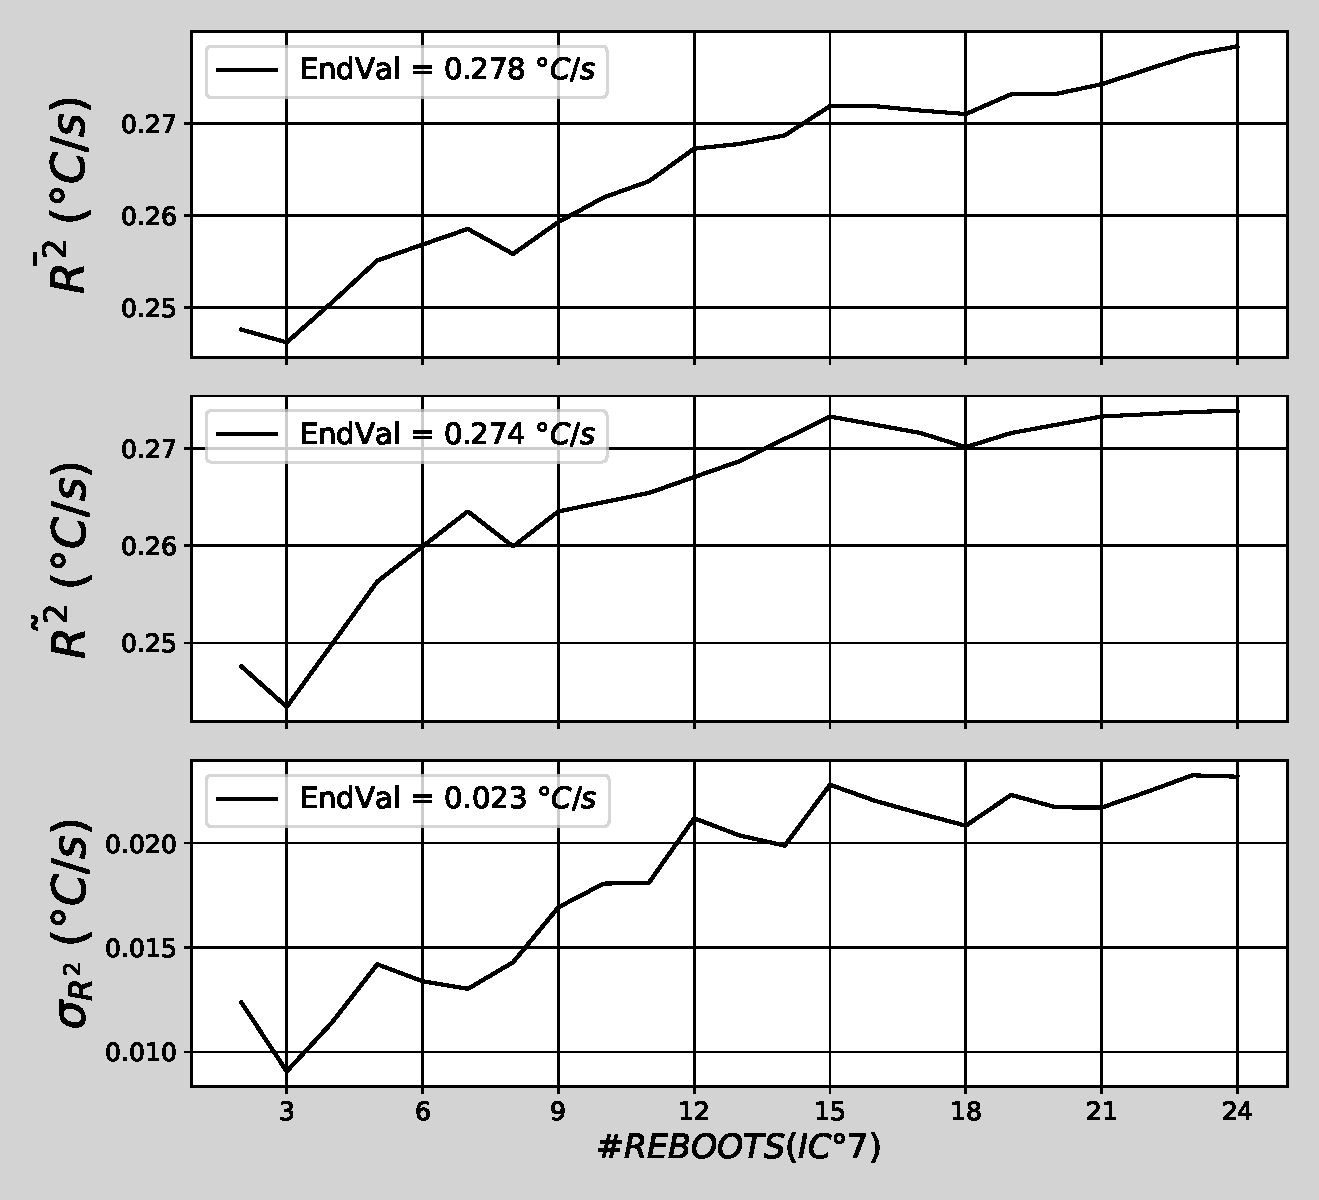
\includegraphics[width=1.0\textwidth]{./figures/flistCircuit7_25_sl30r2.pdf}
		\end{column}
	\end{columns}
\end{frame}

\begin{frame}{STM32 boot: IC8 \textrightarrow\ Opened}
	\vspace{5mm}
	\begin{columns}
		\begin{column}{0.5\textwidth}
			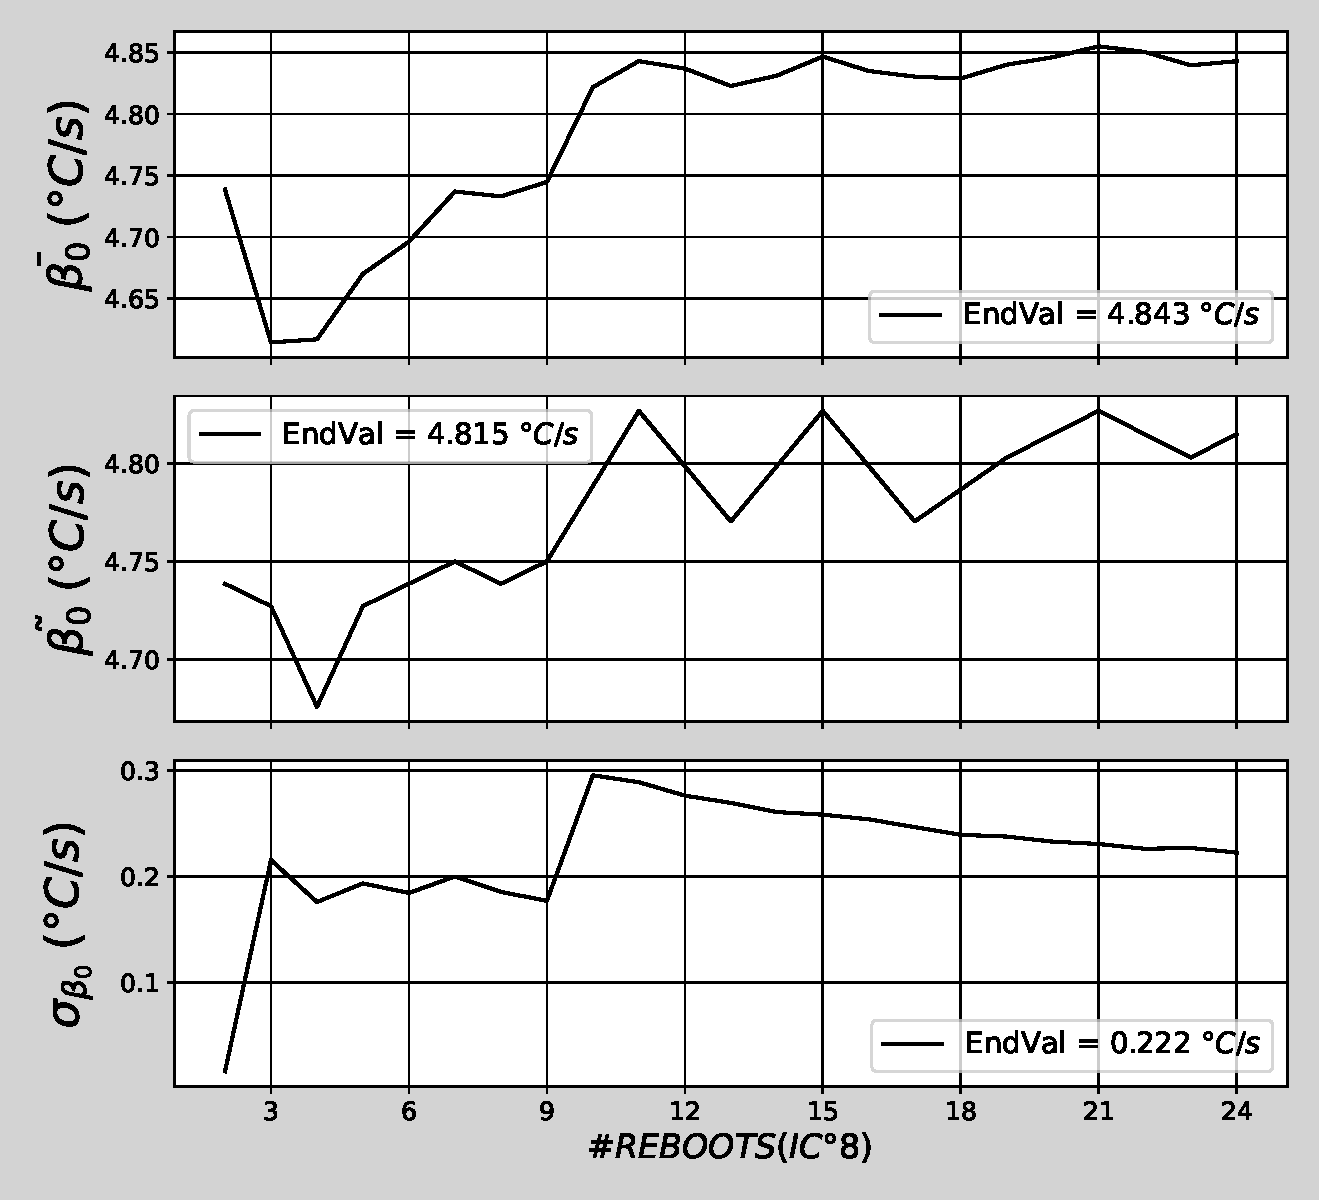
\includegraphics[width=1.0\textwidth]{./figures/flistCircuit8_25_sl30beta0.pdf}
		\end{column}
		\begin{column}{0.5\textwidth}
			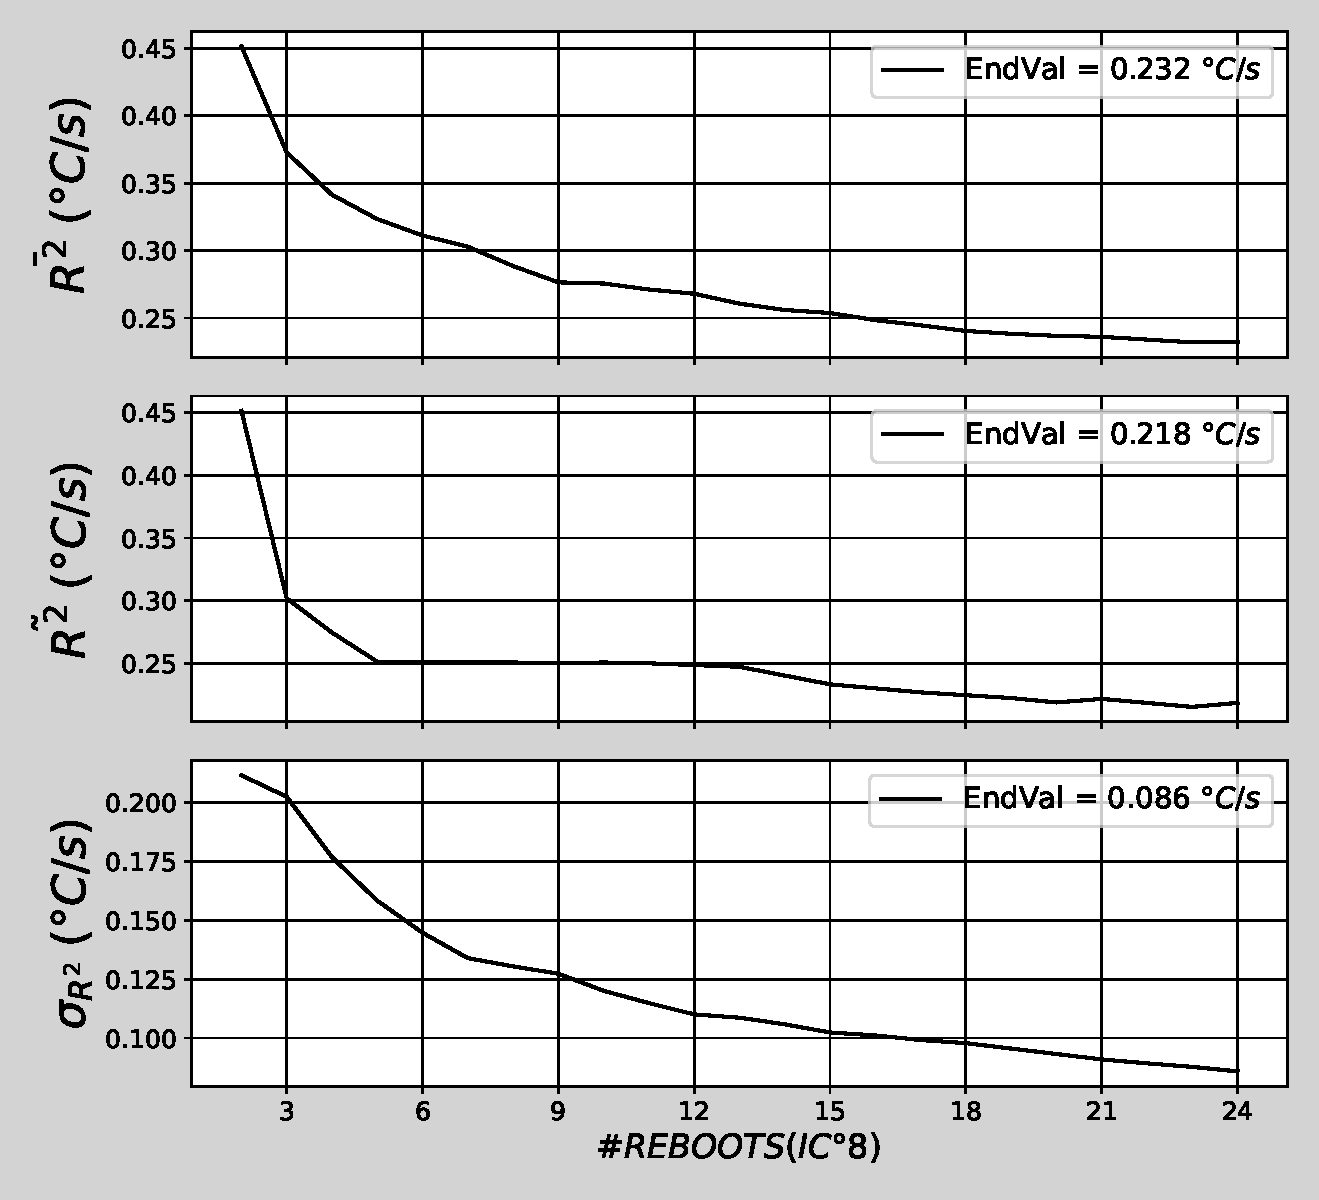
\includegraphics[width=1.0\textwidth]{./figures/flistCircuit8_25_sl30r2.pdf}
		\end{column}
	\end{columns}
\end{frame}

\begin{frame}{STM32 boot: IC9 \textrightarrow\ Opened}
	\vspace{5mm}
	\begin{columns}
		\begin{column}{0.5\textwidth}
			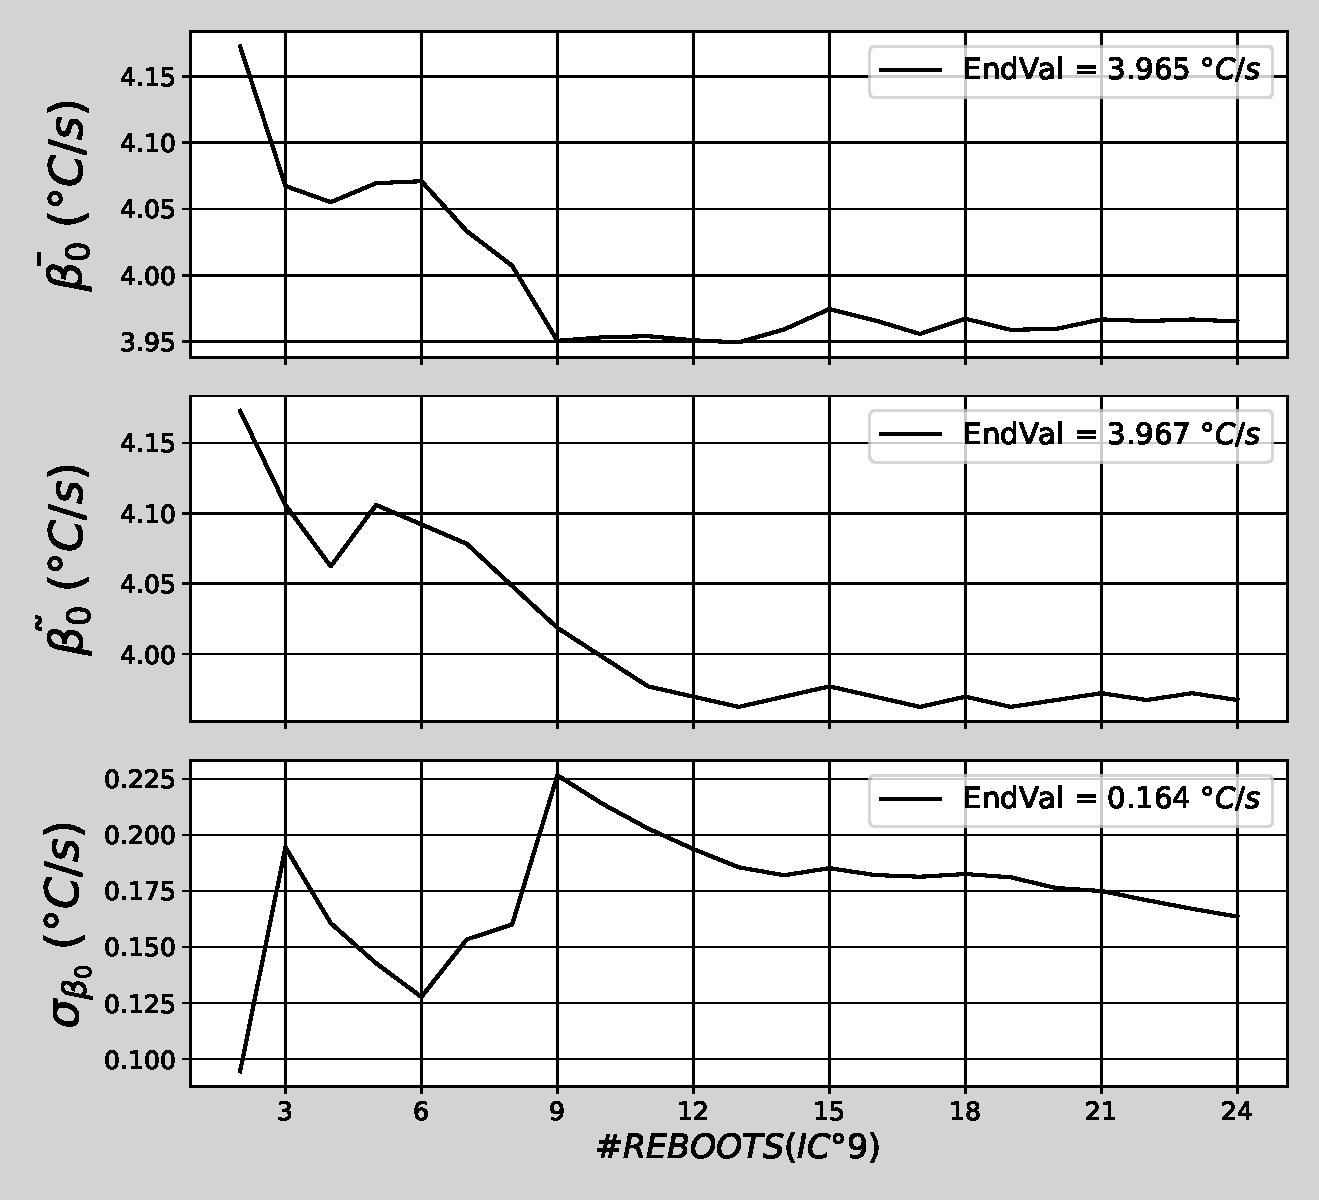
\includegraphics[width=1.0\textwidth]{./figures/flistCircuit9_25_sl30beta0.pdf}
		\end{column}
		\begin{column}{0.5\textwidth}
			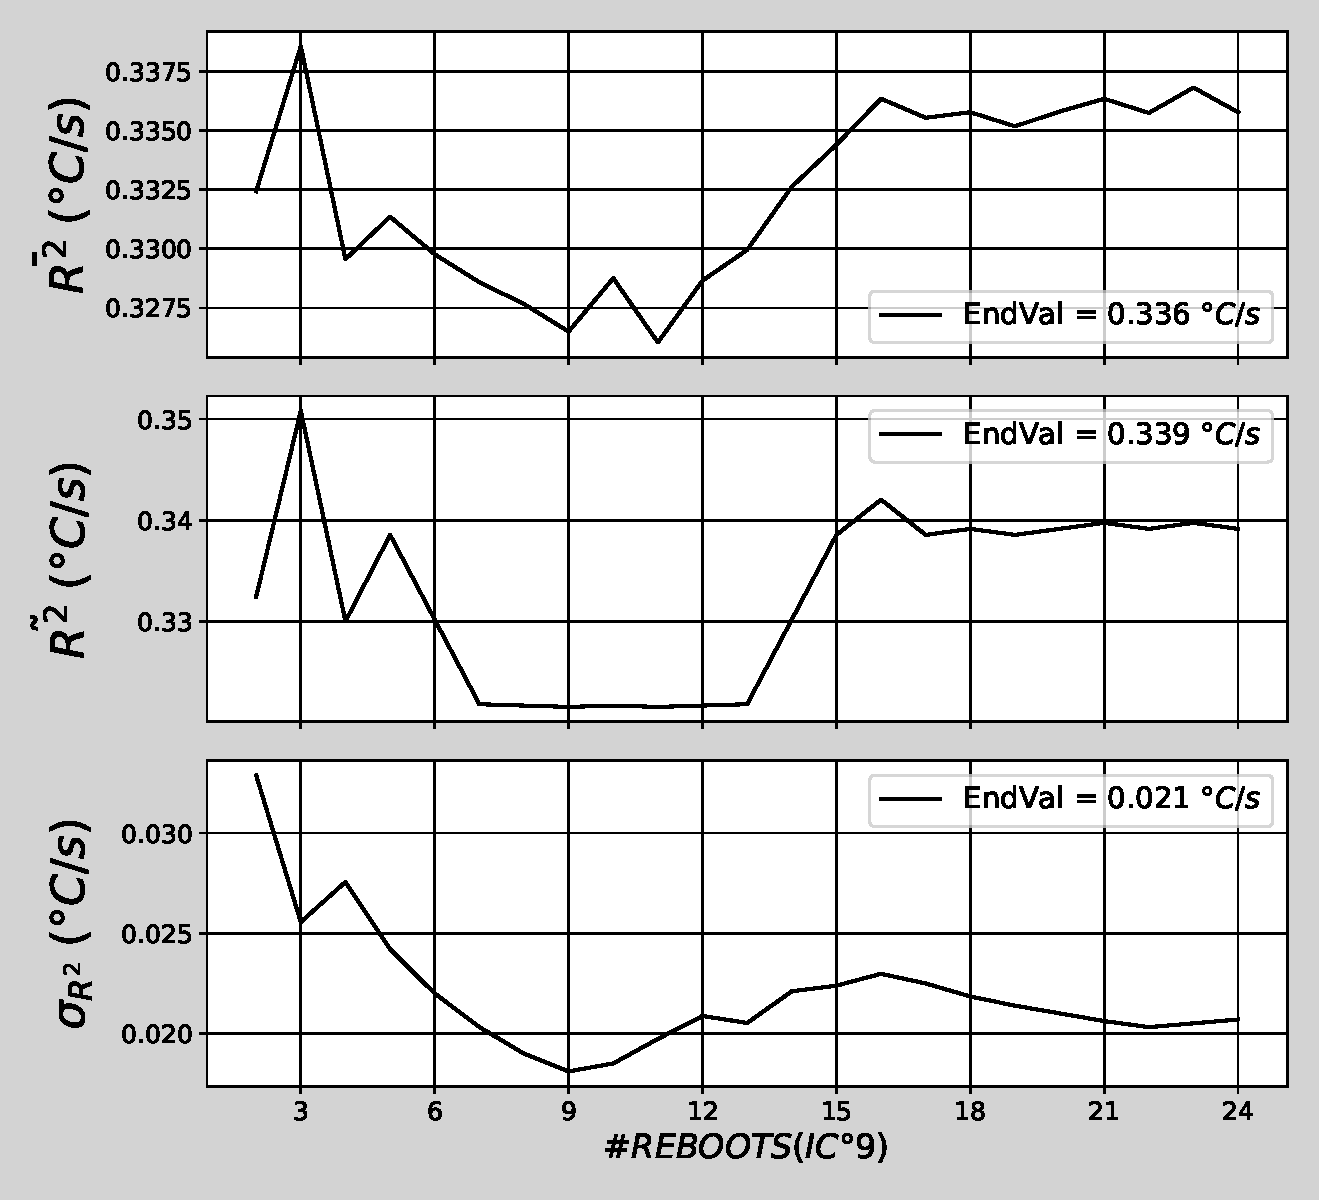
\includegraphics[width=1.0\textwidth]{./figures/flistCircuit9_25_sl30r2.pdf}
		\end{column}
	\end{columns}
\end{frame}

\begin{frame}{STM32 boot: IC10 \textrightarrow\ Opened}
	\vspace{5mm}
	\begin{columns}
		\begin{column}{0.5\textwidth}
			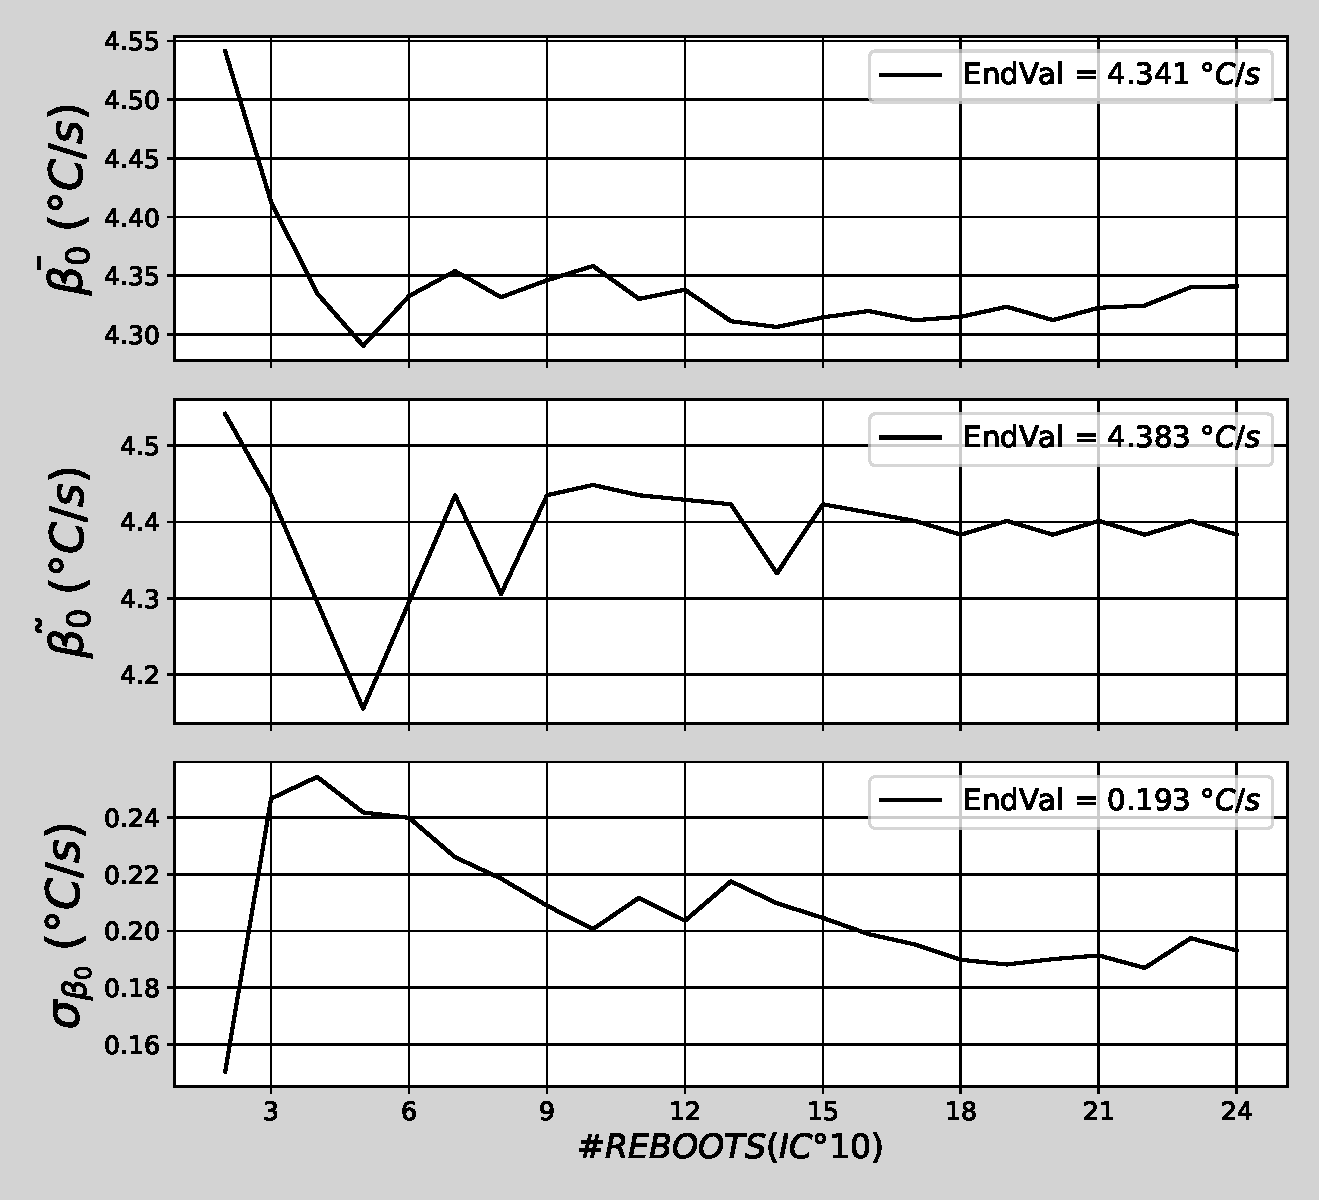
\includegraphics[width=1.0\textwidth]{./figures/flistCircuit10_25_sl5_2beta0.pdf}
		\end{column}
		\begin{column}{0.5\textwidth}
			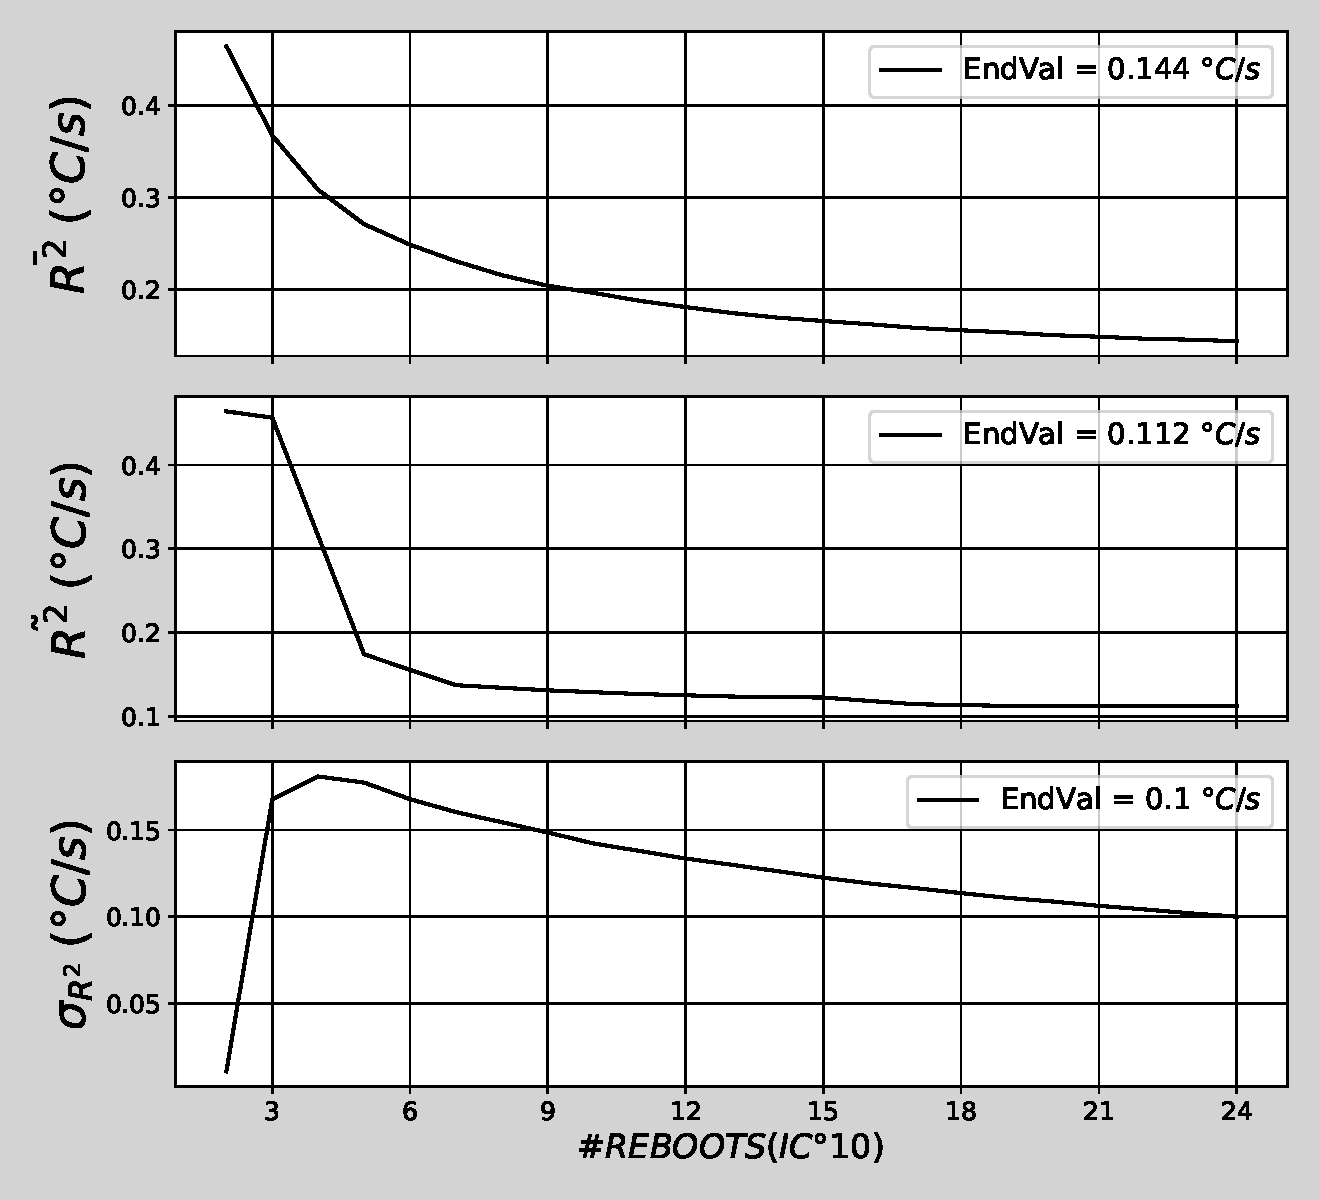
\includegraphics[width=1.0\textwidth]{./figures/flistCircuit10_25_sl5_2r2.pdf}
		\end{column}
	\end{columns}
\end{frame}

\begin{frame}{STM32 boot: IC11 \textrightarrow\ Opened}
	\vspace{5mm}
	\begin{columns}
		\begin{column}{0.5\textwidth}
			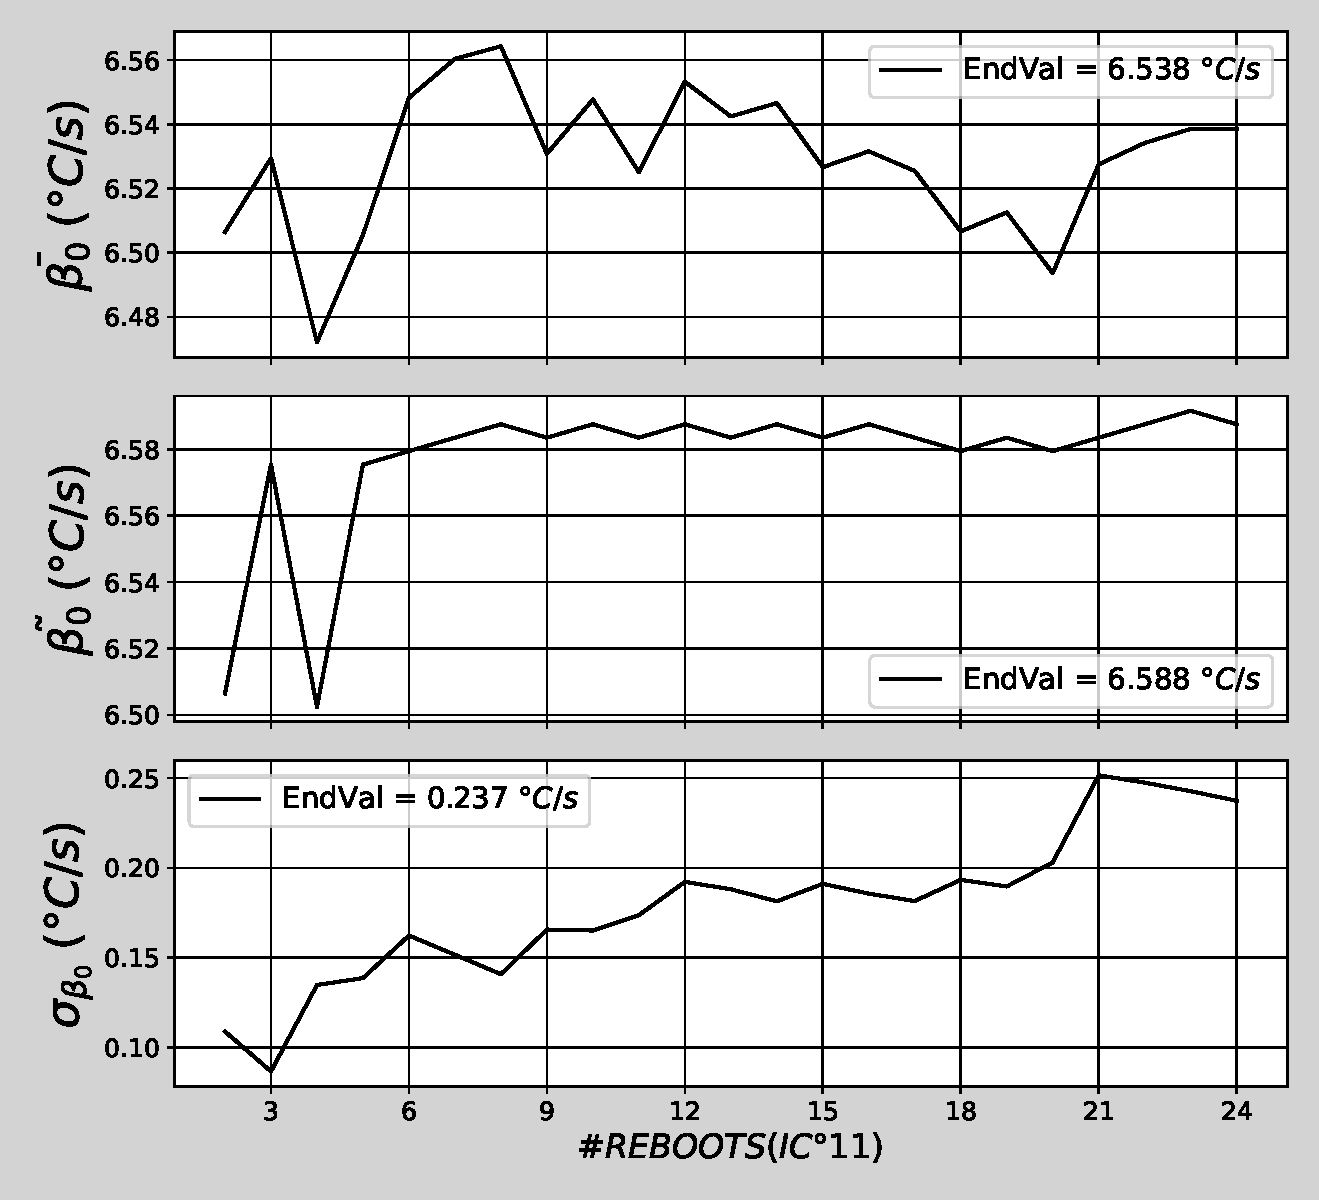
\includegraphics[width=1.0\textwidth]{./figures/flistCircuit11_25_sl30beta0.pdf}
		\end{column}
		\begin{column}{0.5\textwidth}
			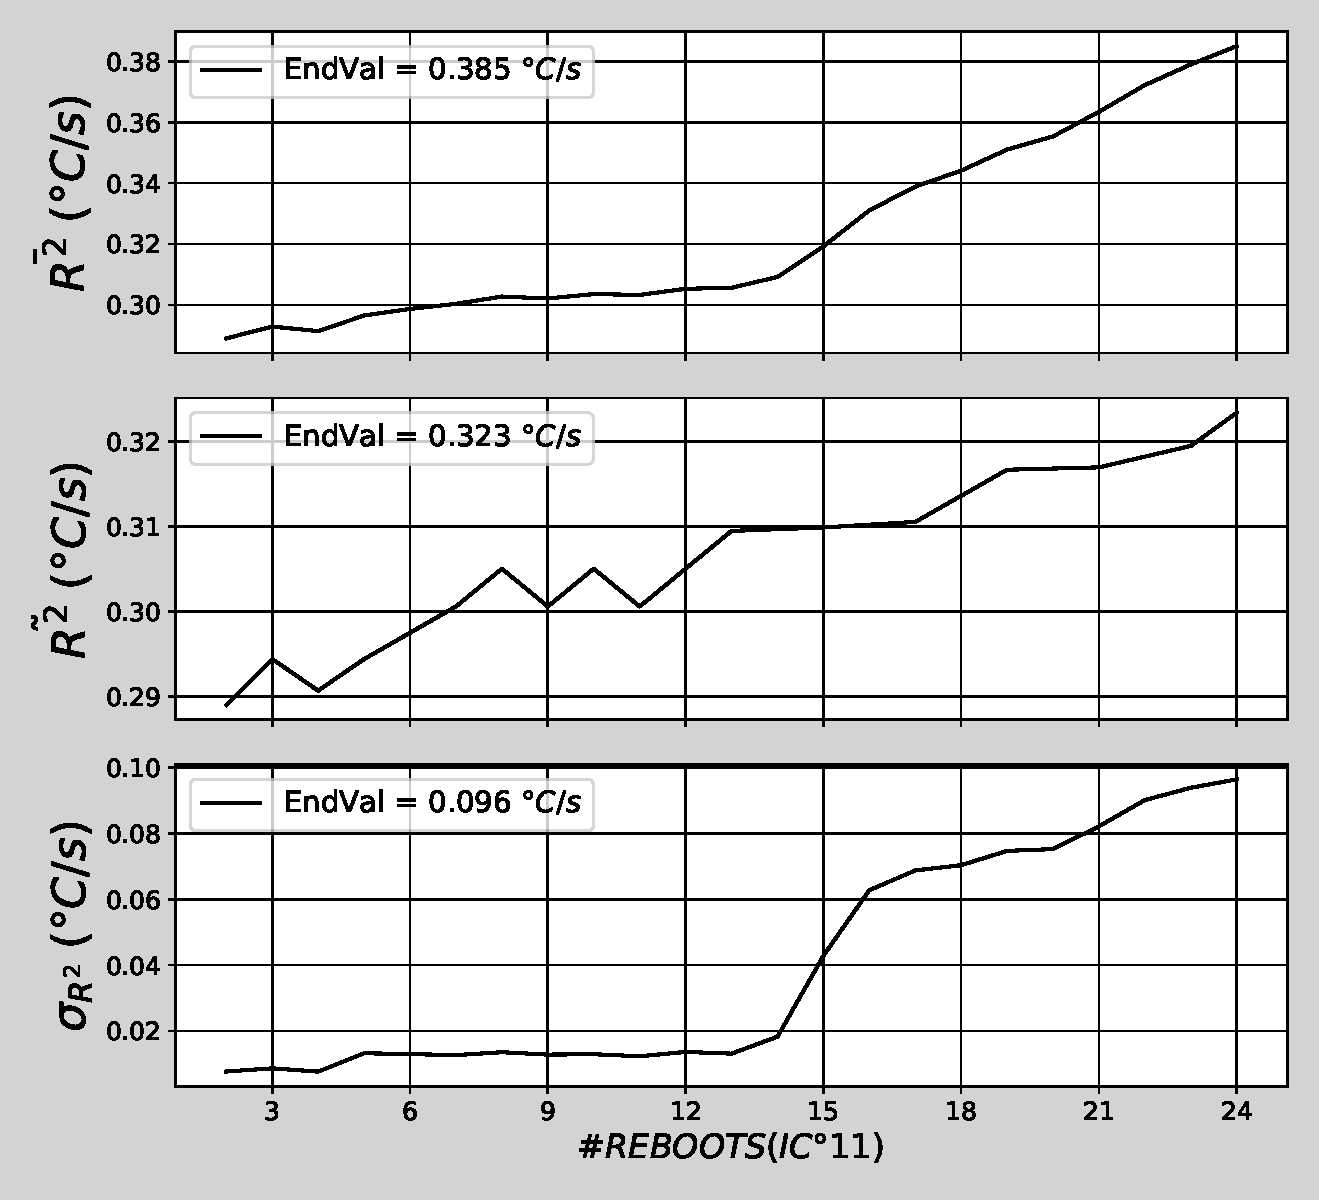
\includegraphics[width=1.0\textwidth]{./figures/flistCircuit11_25_sl30r2.pdf}
		\end{column}
	\end{columns}
\end{frame}

\begin{frame}{STM32 boot: IC12 \textrightarrow\ Closed}
	\vspace{5mm}
	\begin{columns}
		\begin{column}{0.5\textwidth}
			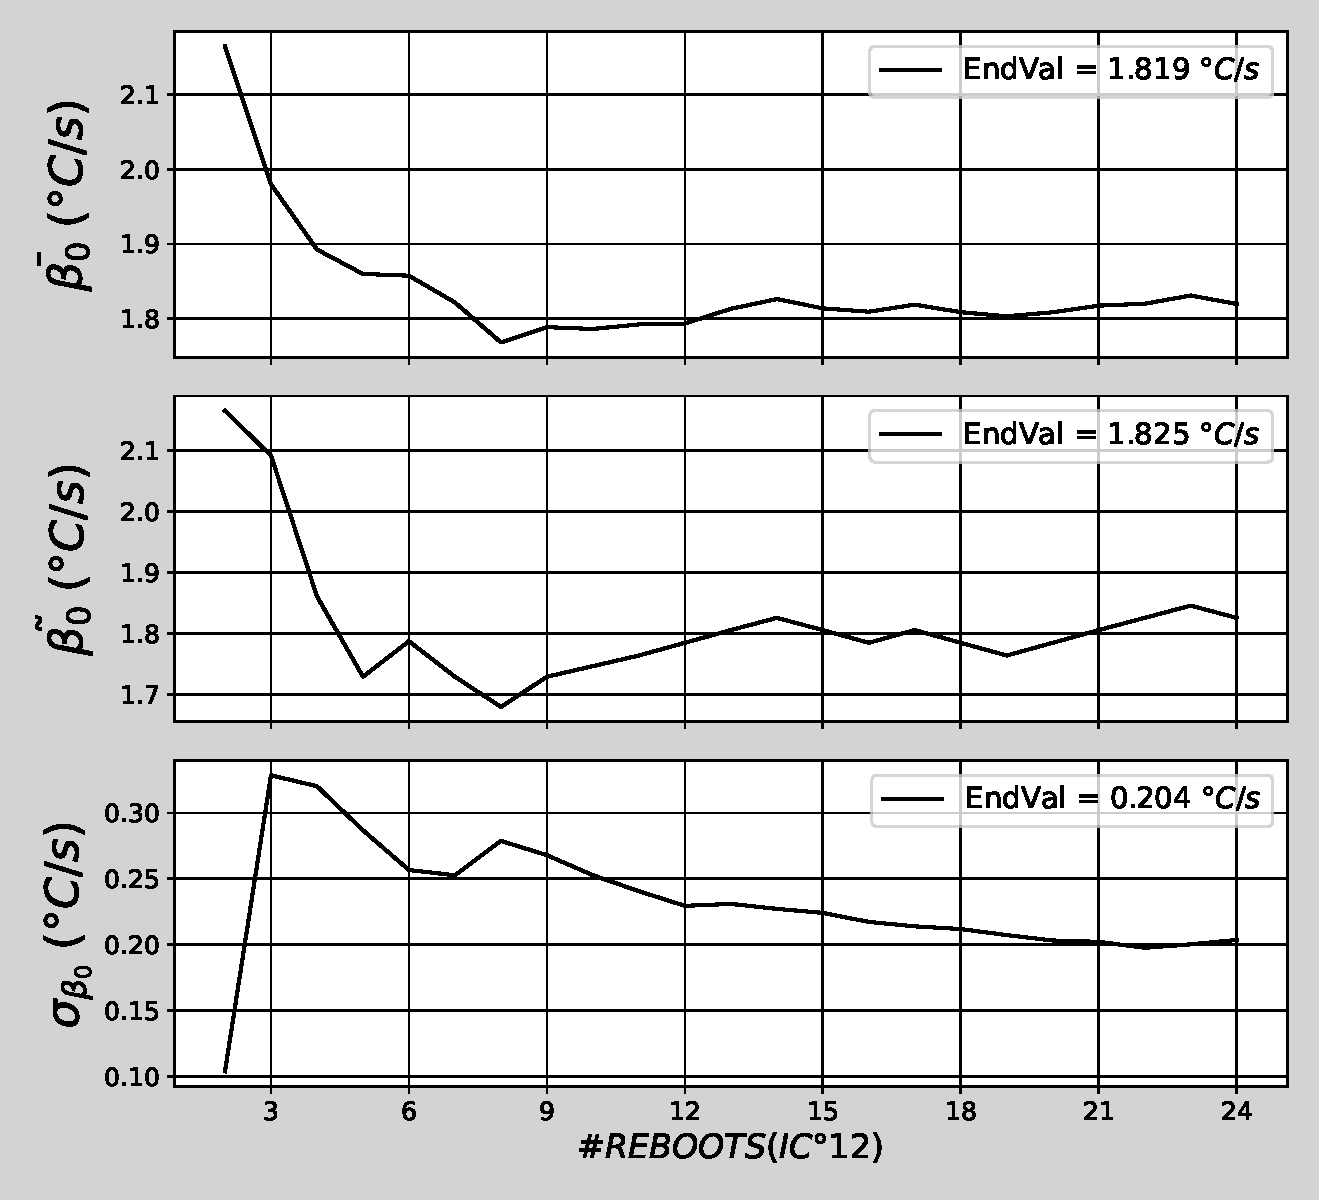
\includegraphics[width=1.0\textwidth]{./figures/flistCircuit12_25_sl30_2beta0.pdf}
		\end{column}
		\begin{column}{0.5\textwidth}
			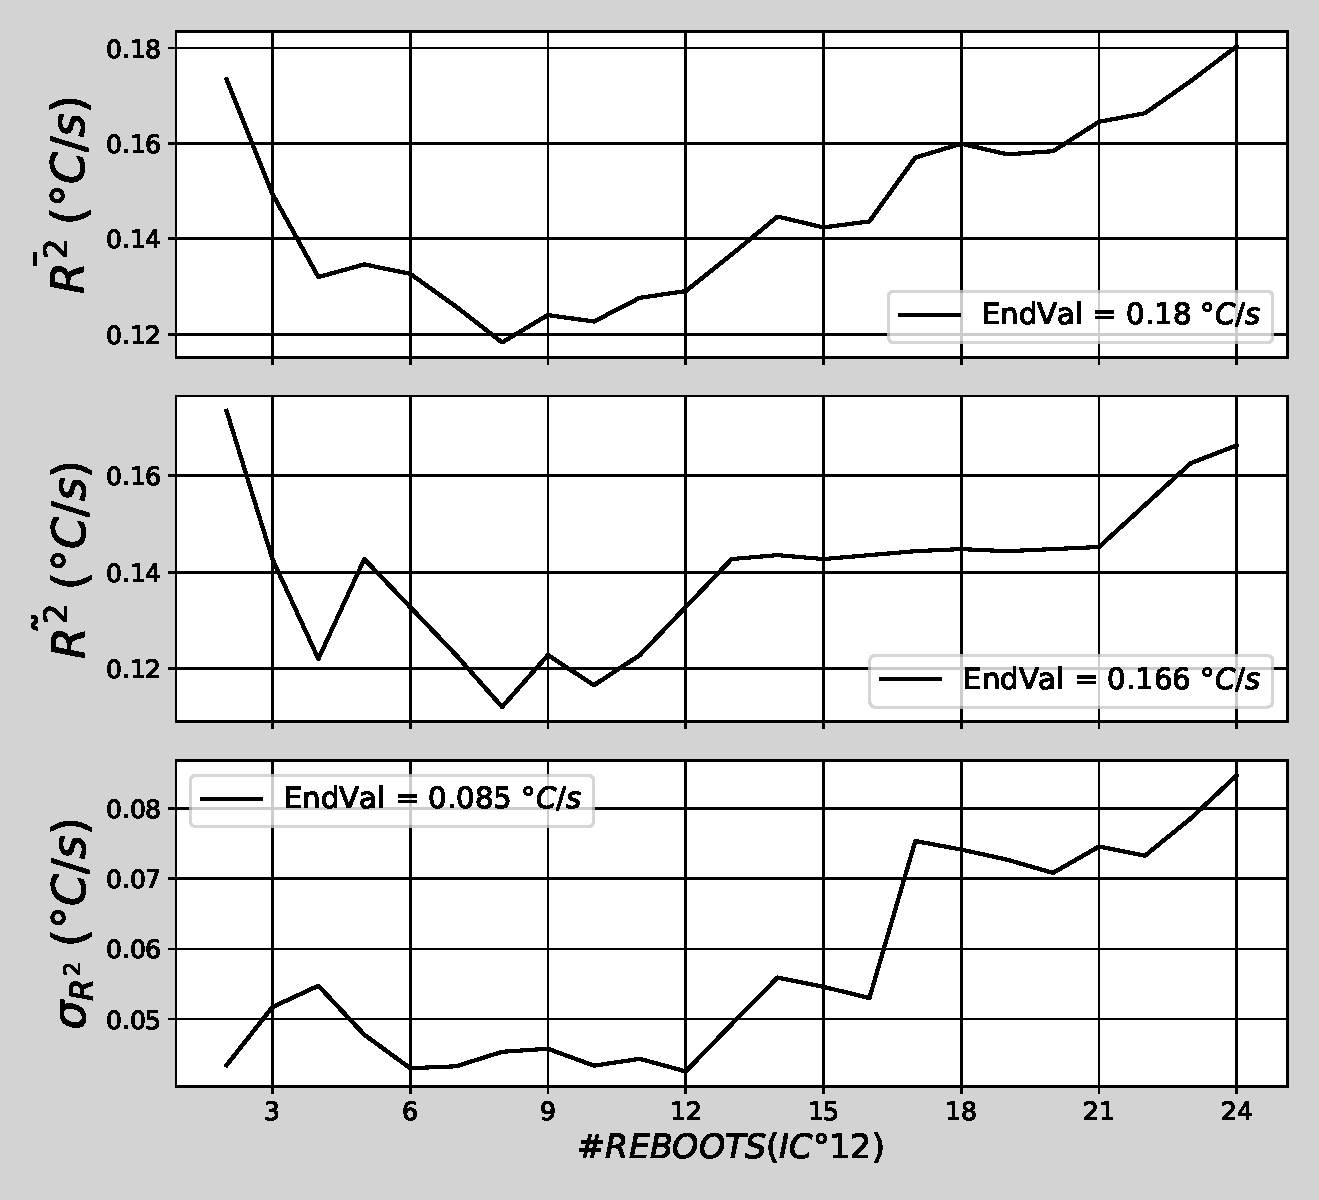
\includegraphics[width=1.0\textwidth]{./figures/flistCircuit12_25_sl30_2r2.pdf}
		\end{column}
	\end{columns}
\end{frame}

\begin{frame}{\textcolor{red}{STM32 boot: IC14 \textrightarrow\ Opened \textrightarrow\ Faulty, discarded}}
	\vspace{5mm}
	\begin{columns}
		\begin{column}{0.5\textwidth}
			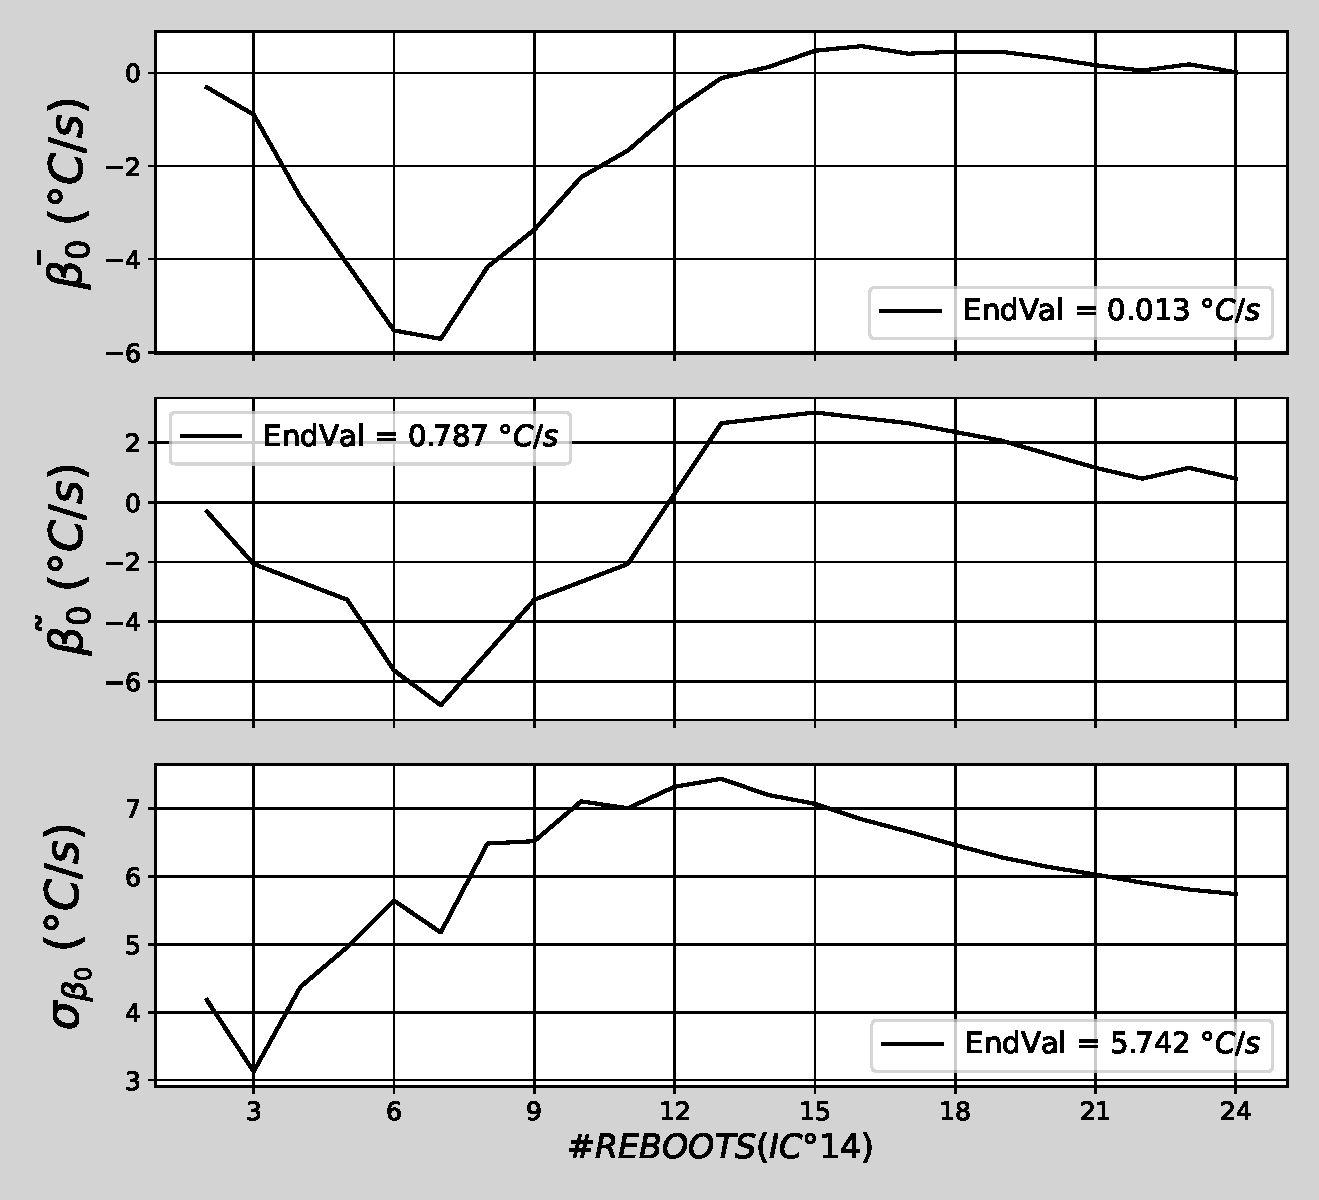
\includegraphics[width=1.0\textwidth]{./figures/flistCircuit14_25_sl30beta0.pdf}
		\end{column}
		\begin{column}{0.5\textwidth}
			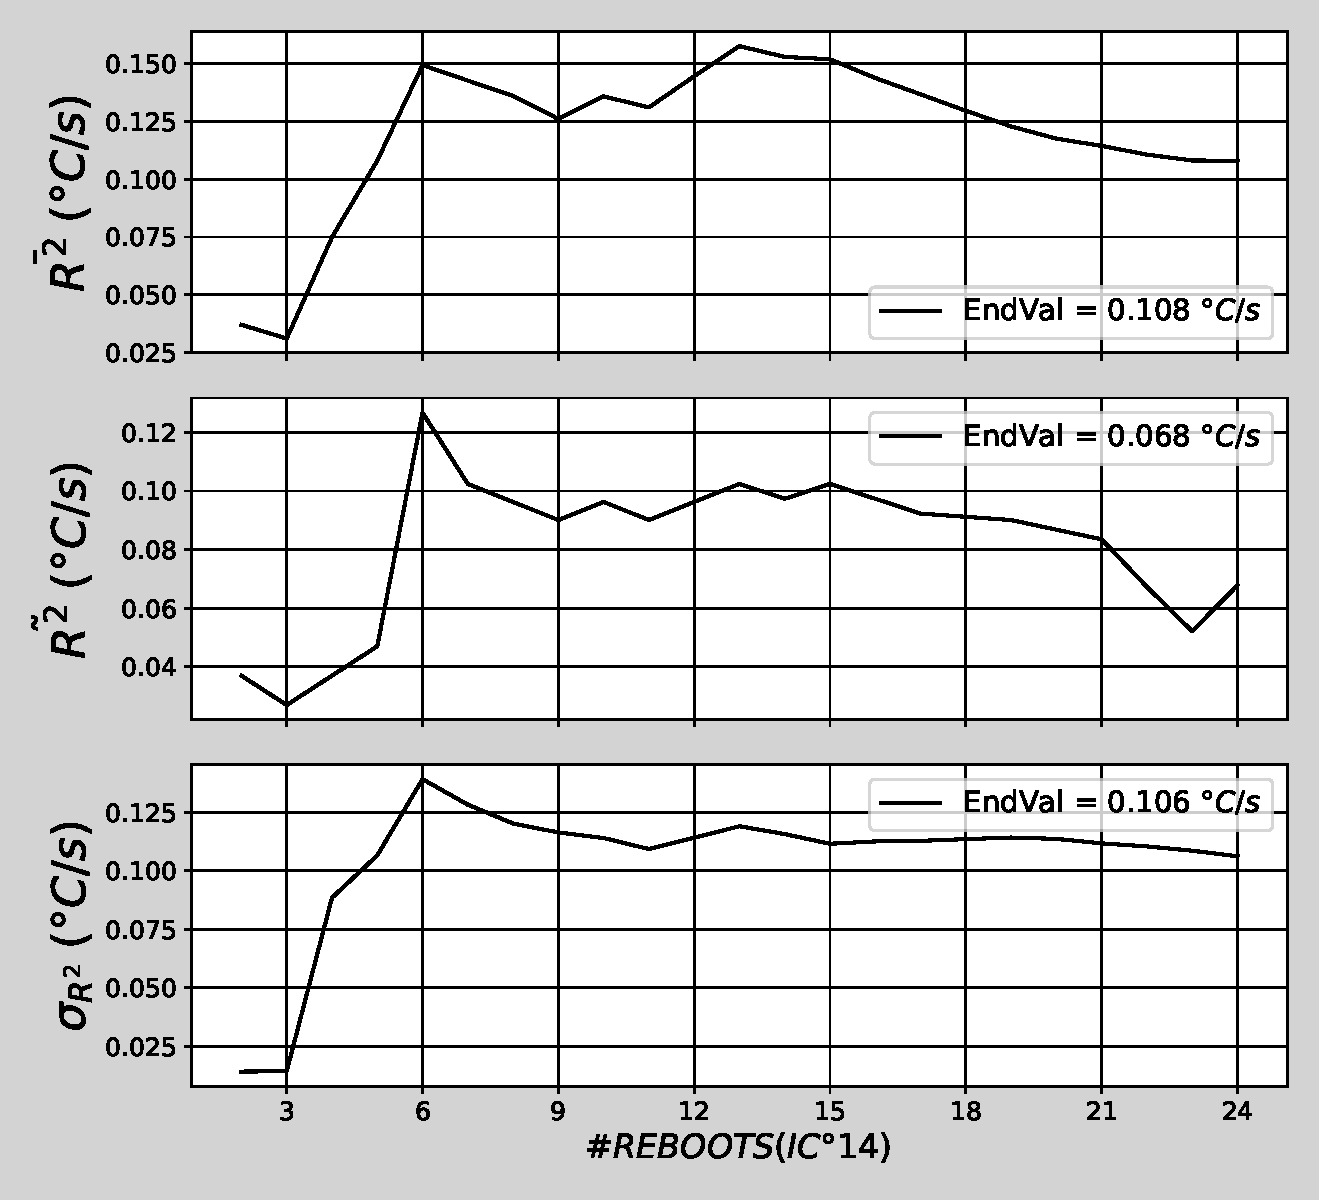
\includegraphics[width=1.0\textwidth]{./figures/flistCircuit14_25_sl30r2.pdf}
		\end{column}
	\end{columns}
\end{frame}

\begin{frame}{STM32 boot: IC25 \textrightarrow\ Closed}
	\vspace{5mm}
	\begin{columns}
		\begin{column}{0.5\textwidth}
			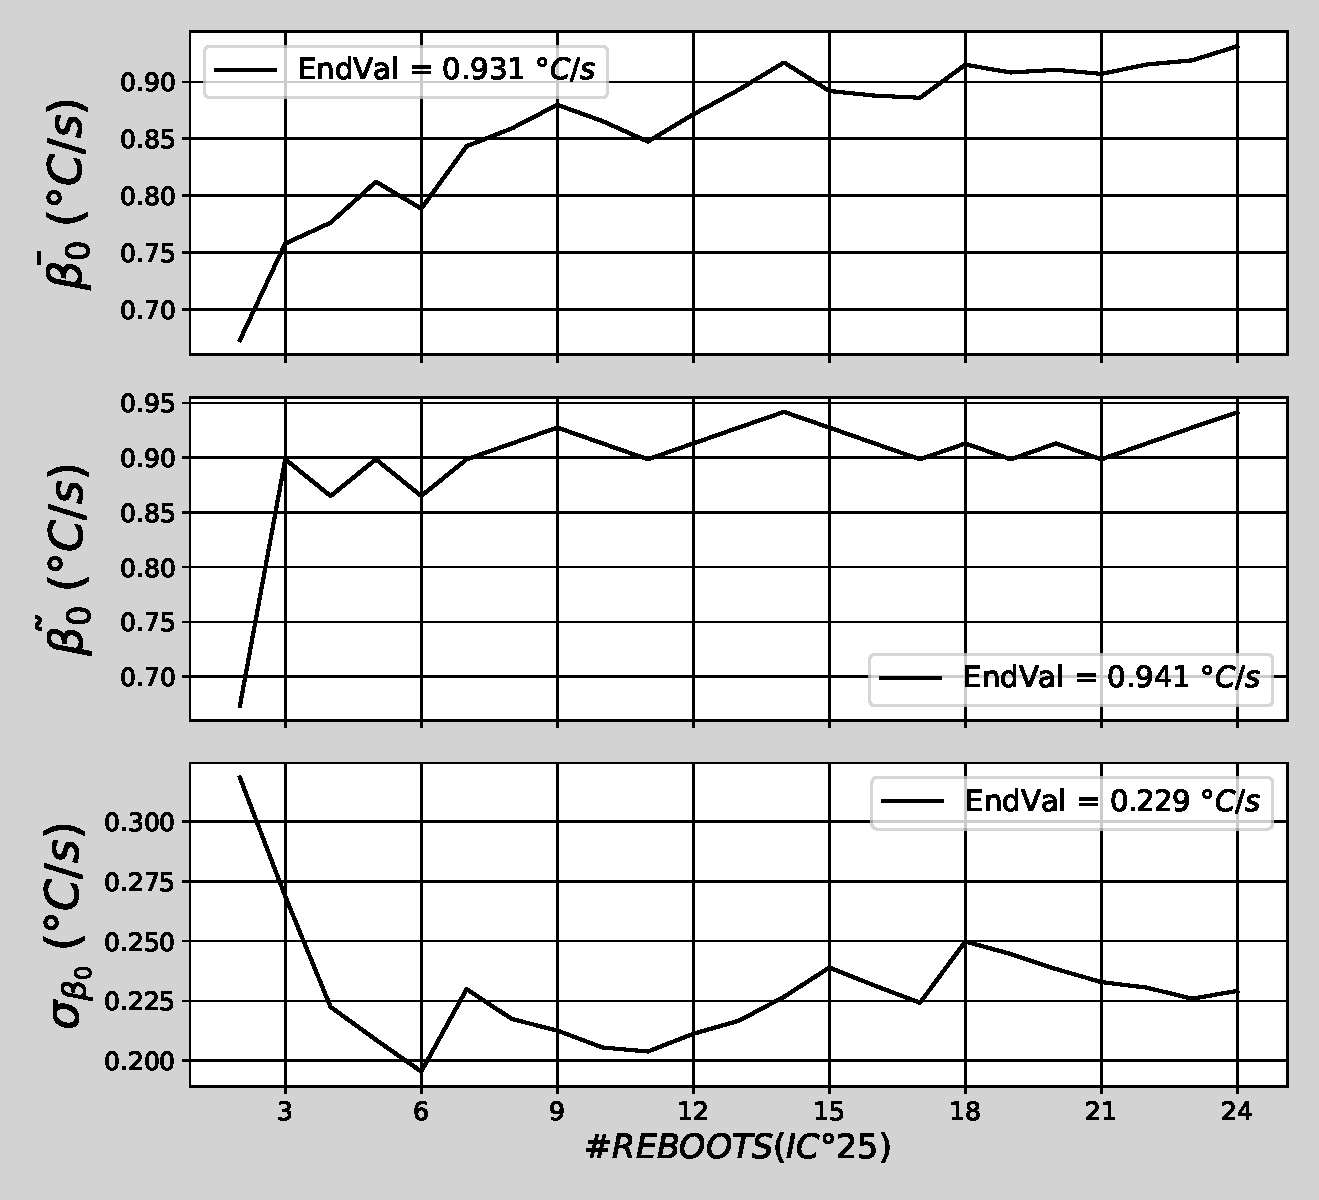
\includegraphics[width=1.0\textwidth]{./figures/flistCircuit25_25_sl30beta0.pdf}
		\end{column}
		\begin{column}{0.5\textwidth}
			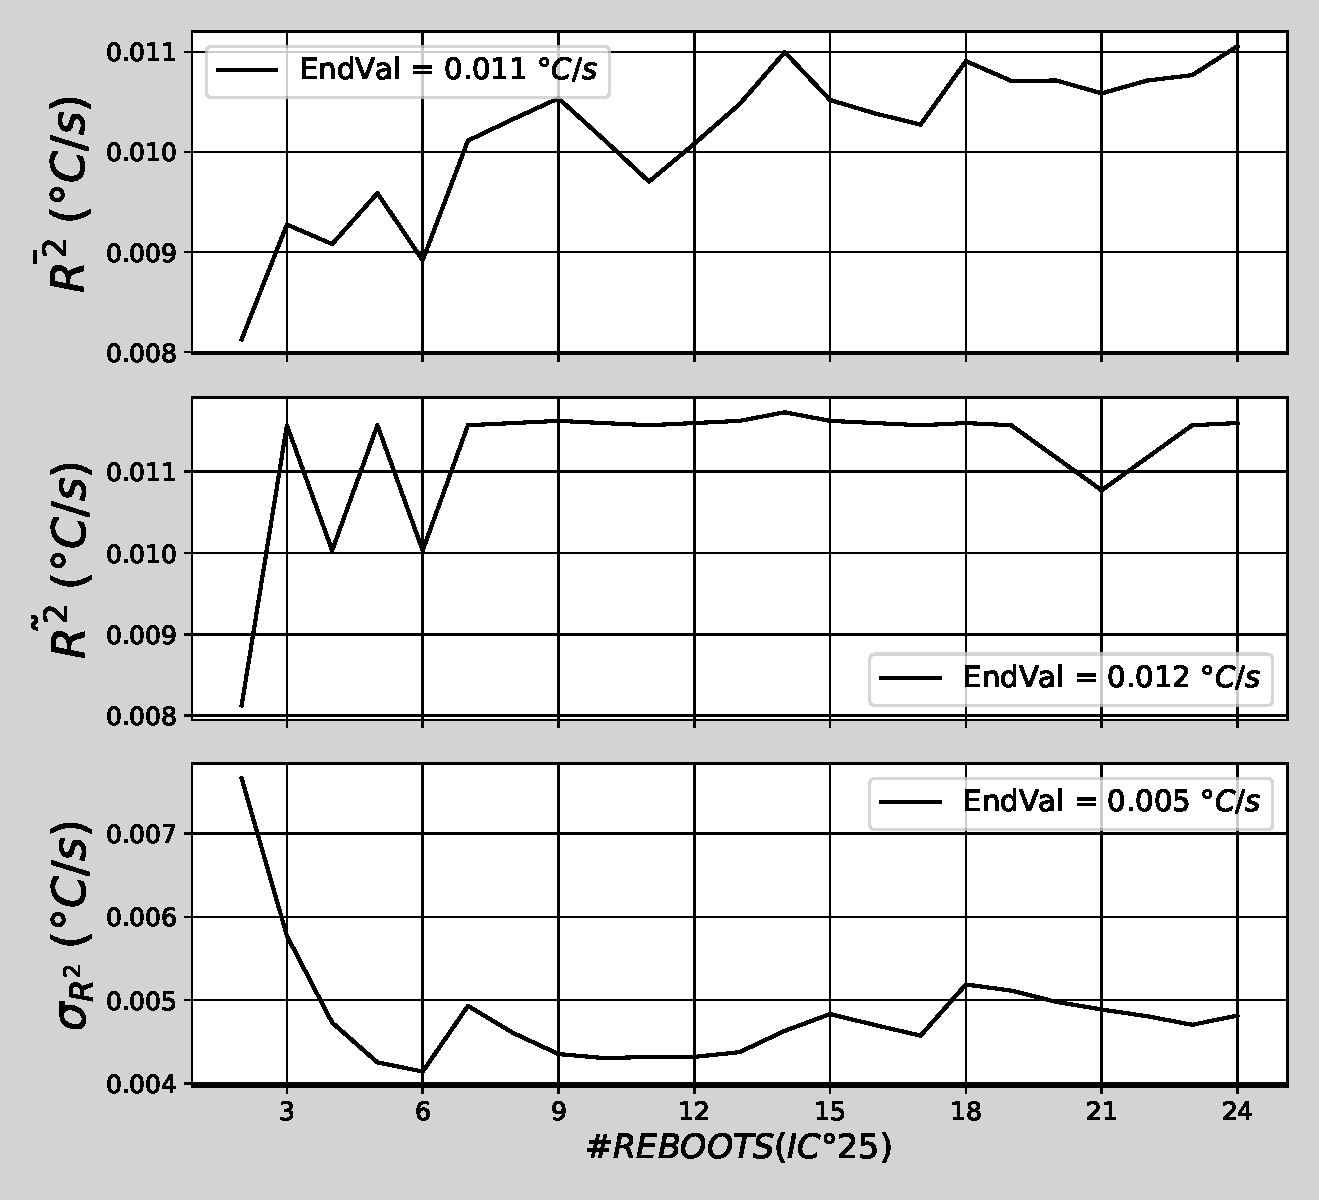
\includegraphics[width=1.0\textwidth]{./figures/flistCircuit25_25_sl30r2.pdf}
		\end{column}
	\end{columns}
\end{frame}

\begin{frame}{STM32 boot: IC26 \textrightarrow\ Closed}
	\vspace{5mm}
	\begin{columns}
		\begin{column}{0.5\textwidth}
			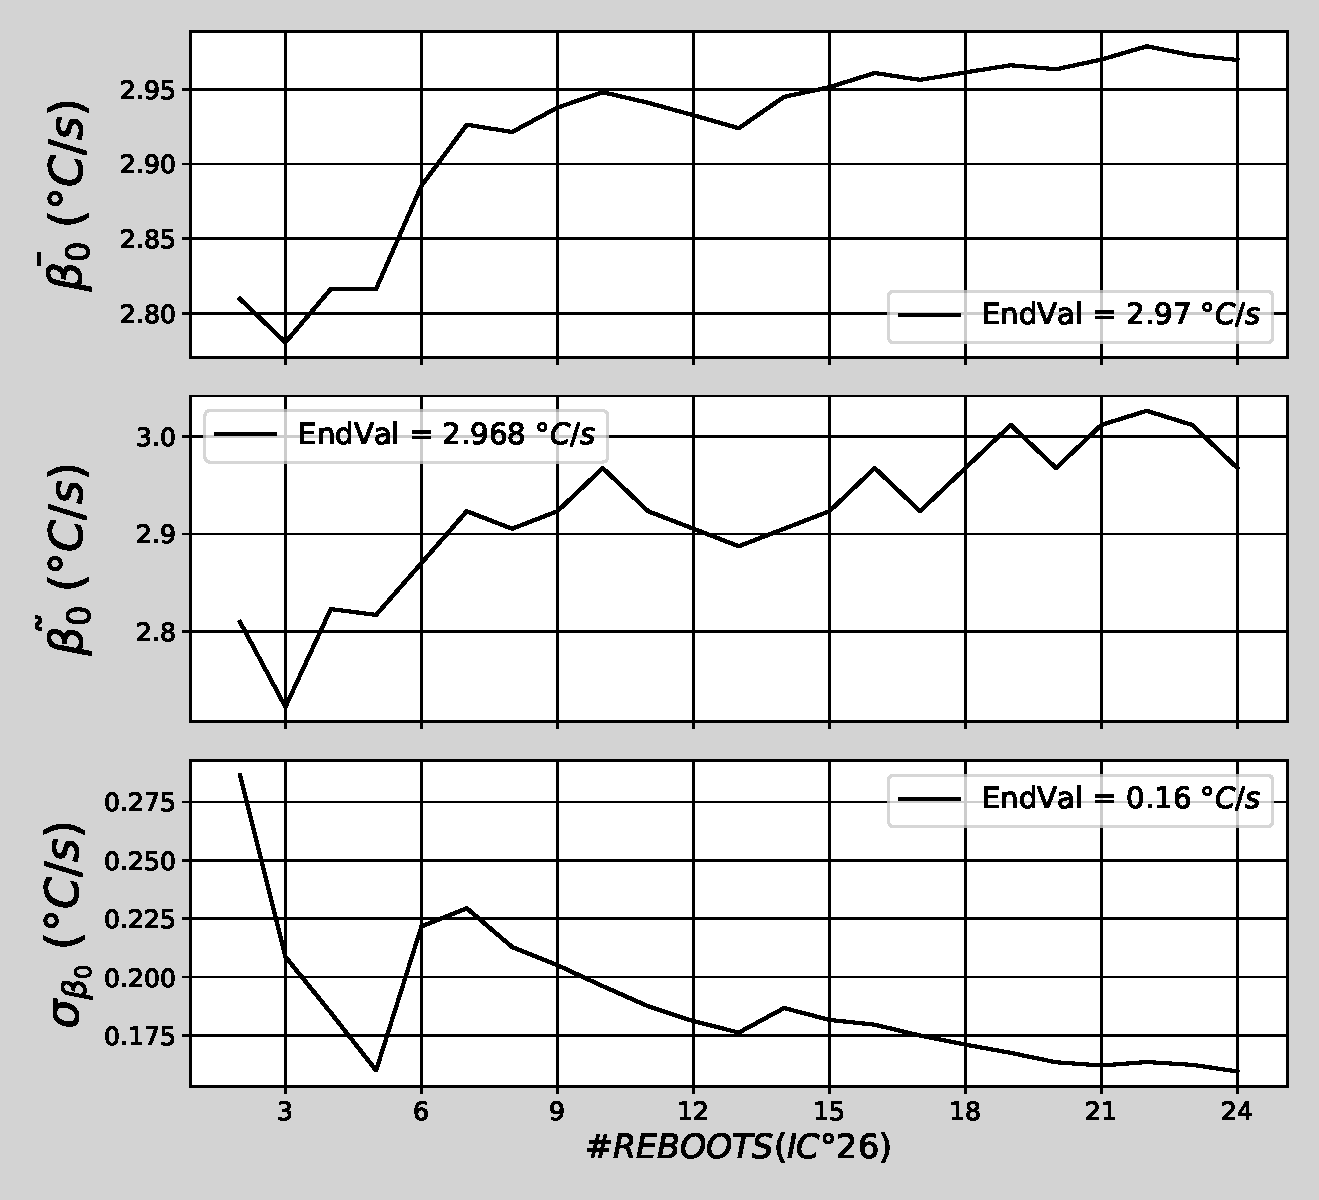
\includegraphics[width=1.0\textwidth]{./figures/flistCircuit26_25_sl30beta0.pdf}
		\end{column}
		\begin{column}{0.5\textwidth}
			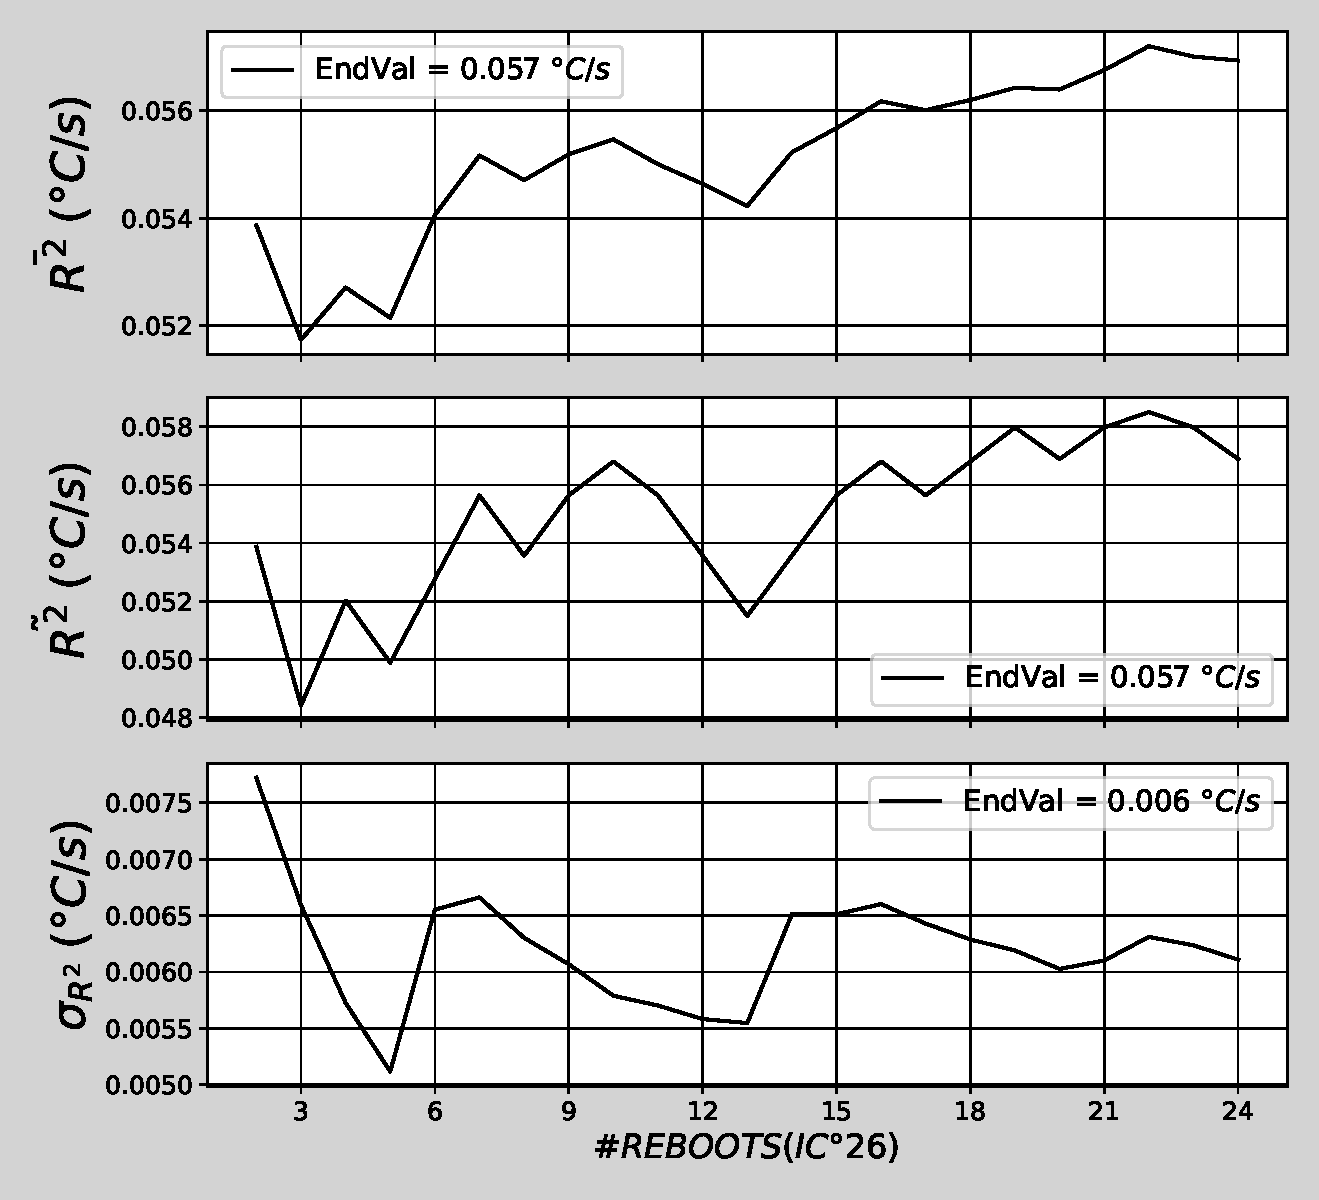
\includegraphics[width=1.0\textwidth]{./figures/flistCircuit26_25_sl30r2.pdf}
		\end{column}
	\end{columns}
\end{frame}

	% !TeX root = ./0_slides.tex

\begin{frame}{STM32 boot: summary}
	\vspace{-3mm}
	\begin{table}[]
		\centering
		\begin{tabular}{|l|l|l|l|l|l|}
			\hline \rule{0pt}{12pt} IC n\textsuperscript{o} & $\bar{\beta_0} \; (^{\circ} C/s)$ & $\sigma_{\beta_0} \; (^{\circ} C/s)$ & $\bar{R^2} \; (^{\circ} C/s)$ & $\sigma_{R^2} \; (^{\circ} C/s)$ & Backside \\ \hline
			25       & 0.931  & 0.229  & 0.011    &  0.005    & Closed           \\ \hline
			3         & 1.405  & 0.145  & 0.06      &  0.015    & Closed            \\ \hline
			12       & 1.819  & 0.204  & 0.18      &	0.085  & Closed            \\ \hline
			6         & 2.183  & 0.191  & 0.08      &	0.012   & Closed            \\ \hline
			2         & 2.503  & 0.322  & 0.174    &  0.146    & Closed            \\ \hline
			26       & 2.97    & 0.16    & 0.057    &  0.006    & Closed            \\ \hline
			1         & 3.433  & 0.159  & 0.093    &  0.08      & Opened         \\ \hline
			9         & 3.965  & 0.167  & 0.336    &  0.021    & Opened         \\ \hline
			10       & 4.341  & 0.193  & 0.144    &  0.1        & Opened         \\ \hline
			7         & 4.567  & 0.137  & 0.278    &  0.023    & Opened         \\ \hline
			8         & 4.843  & 0.222  & 0.232    &  0.086    & Opened         \\ \hline
			4         & 6.351  & 0.149  & 0.437    &  0.078    & Opened         \\ \hline
			11       & 6.539  & 0.237  & 0.385    &  0.096    & Opened         \\ \hline
		\end{tabular}
	\end{table}
\end{frame}

\begin{frame}{STM32 boot: heatsink with 7 backside opened ICs}
%	\vspace{-3mm}
	\begin{columns}
		\begin{column}{0.5\textwidth}
			\centering
			Open-air backside
			\begin{table}[]
				\centering
				\begin{tabular}{|l|l|l|}
					\hline \rule{0pt}{12pt} IC n\textsuperscript{o} & $\bar{\beta_0} \; (^{\circ} C/s)$ & $\sigma_{\beta_0} \; (^{\circ} C/s)$  \\ \hline
					1         & 3.433  & 0.159    \\ \hline
					9         & 3.965  & 0.167    \\ \hline
					10       & 4.341  & 0.193    \\ \hline
					7         & 4.567  & 0.137    \\ \hline
					8         & 4.843  & 0.222    \\ \hline
					4         & 6.351  & 0.149    \\ \hline
					11       & 6.539  & 0.237    \\ \hline
				\end{tabular}
			\end{table}
		\end{column}
		\begin{column}{0.5\textwidth}
			\centering
			Heat-sunk backside
			\begin{table}[]
				\centering
				\begin{tabular}{|l|l|l|}
					\hline \rule{0pt}{12pt} IC n\textsuperscript{o} & $\bar{\beta_0} \; (^{\circ} C/s)$ & $\sigma_{\beta_0} \; (^{\circ} C/s)$  \\ \hline
					1         & 0.831  & 0.222    \\ \hline
					9         & 0.976  & 0.172    \\ \hline
					10       & 0.203  & 0.122    \\ \hline
					7         & 1.728  & 0.161    \\ \hline
					8         & 2.771  & 0.853    \\ \hline
					4         & 4.139  & 0.311    \\ \hline
					11       & 2.996  & 0.213    \\ \hline
				\end{tabular}
			\end{table}
		\end{column}
	\end{columns}
\end{frame}

	
\end{document}
